\documentclass[12pt]{report}
\usepackage{cdtUsecases}
\usepackage[utf8]{inputenc}
\usepackage{hyperref}
\usepackage{txfonts}
\usepackage{graphicx}
\usepackage{float}
\usepackage{enumerate} 
\usepackage{wrapfig}
\usepackage{eso-pic}
\usepackage{wallpaper} 

\newcommand\BackgroundPic{
		\parbox[b][\paperheight]{\textwidth}{%
			\vfill
			\flushleft
			
\includegraphics[width=0.18\paperwidth,height=\paperheight,
			keepaspectratio]{images/port2}%
			\vfill
}}
\newenvironment{changemargin}[2]{% 
	\begin{list}{}{% 
			\setlength{\topsep}{0pt}% 
			\setlength{\leftmargin}{#1}% 
			\setlength{\rightmargin}{#2}% 
			\setlength{\listparindent}{\parindent}% 
			\setlength{\itemindent}{\parindent}% 
			\setlength{\parsep}{\parskip}% 
		}% 
		\item[]}{\end{list}} 
%%%%%%%%%%%%%%%%%%%%%%%%%%%%%%%%%%%%%%%%%%%%%%%%%%%%%%%%%%%%%%%%
\begin{document}	
	\AddToShipoutPicture*{\BackgroundPic}
	\begin{center}
	\vspace*{0.4in}
\begin{LARGE}
	\textbf {INSTITUTO POLITÉCNICO NACIONAL}\\
\end{LARGE}
\smallskip
\begin{large}
	\textbf {ESCUELA SUPERIOR DE CÓMPUTO}\\
\end{large}
\vspace*{0.35in}
\begin{LARGE}
	\textbf {ESCOM}\\
\end{LARGE}
	\vspace*{0.5in}
\begin{large}	
\textit {Trabajo terminal}\\
\end{large}
	\vspace*{0.3in}
\begin{Large}	
	\textbf {Sistema generador de documentos de casos de uso\\
		"TESSERACT"}\\
\end{Large}
\bigskip
\begin{large}	
	\textit {2018-B140}\\
\end{large}
	\vspace*{0.3in}
\begin{large}	
	\textit {Presentan}\\
	\textbf {Jiménez Chávez Luis Gerardo}\\
	\textbf {López Orozco Diego Efrain}\\
	\textbf {Martínez Ibáñez Esteban Pablo}\\
	\textbf {Olvera Neria Yamile Giselle}\\
\end{large}
	\vspace*{0.3in}
\begin{large}	
	\textit {Directores}\\
\end{large}

\begin{normalsize}
	\textbf {M. en C. Hermes Francisco \hspace{1.5cm} M. en C. José Jaime\\
	.\hspace{0.5cm} Montes Casiano \hspace{2.8cm} López Rabadán }
\end{normalsize}

\end{center}
\vspace*{0.8in}
\begin{flushright}
noviembre del 2019
\end{flushright}

\newpage

\begin{figure}[H]
	\begin{minipage}[p]{0.13\linewidth}
		\centering
		
\includegraphics[width=\linewidth]{images/logoIPN}
	\end{minipage}
	\hspace{.85cm}
\begin{minipage}[p] {0.55\linewidth}
	\begin{center}
		\begin{large}
			\textbf {INSTITUTO POLITÉCNICO NACIONAL}\\
			\textbf {ESCUELA SUPERIOR DE CÓMPUTO}\\
			\textbf {SUBDIRECCIÓN ACADÉMICA}\\
		\end{large}
	\end{center}
\end{minipage}
	\hspace{.85cm}
	\begin{minipage}[p]{0.20\linewidth}
		\centering
		
\includegraphics[width=\linewidth]{images/logoESCOM}
	\end{minipage}
\end{figure}

\begin{normalsize}
No de TT:2018-B140 \hspace{10cm} noviembre de 2019
\end{normalsize}

\begin{center}
	\begin{normalsize}
		Documento Técnico\\
	\end{normalsize}
	\vspace*{0.2in}	
	\begin{large}
		\textbf {Sistema generador de documentos de casos de uso\\
			"TESSERACT"}\\
	\end{large}
	\vspace*{0.3in}
	\begin{large}	
		\textit {Presentan}\\
		\textbf {Jiménez Chávez Luis Gerardo} \hyperlink{x01}{[1]}\\
		\textbf {López Orozco Diego Efrain} \hyperlink{x02}{[2]}\\
		\textbf {Martínez Ibáñez Esteban Pablo} \hyperlink{x03}{[3]}\\
		\textbf {Olvera Neria Yamile Giselle} \hyperlink{x04}{[4]}\\
	\end{large}
	\vspace*{0.3in}
	\begin{large}	
		\textit {Directores}\\
	\end{large}
	
	\begin{normalsize}
		\textbf {M. en C. Hermes Francisco \hspace{1.5cm} M. en C. José Jaime\\
			.\hspace{0.6cm} Montes Casiano \hspace{2.8cm} López Rabadán }
	\end{normalsize}
	\vspace*{0.3in}
	\begin{large}	
	\textbf {RESUMEN}\\
	\end{large}
\end{center}
	\begin{normalsize}
		En este reporte se presenta la documentación técnica del Trabajo Terminal 2018-B140 titulado
		"Sistema generador de documentos de casos de uso", cuyo objetivo es desarrollar un sistema web que asista en la generación de la documentación de casos de uso de un proyecto de software con base en una plantilla predefinida a fin de contribuir en su proceso de creación.\\ 	
	\end{normalsize}
	\begin{small}
		Palabras clave: Administración de Proyectos, Ciclo de vida del software, Documento de caso de uso, Ingeniería de Software, Lenguaje Unificado de Modelado (UML)\\
	\end{small}
\begin{scriptsize}
    \_\_\_\_\_\_\_\_\_\_\_\_\_\_\_\_\_\_\_\_\_\_\_\_\_\_\_\_\_\_\_\_\_\_\_\_\_\_\_\_\_\_\_\_\_\_\_\_ \\
    Correos electrónicos:\\
	\hypertarget{x01}{[1]} lgjc1im11@gmail.com \\
	\hypertarget{x01}{[2]} quakediego33@hotmail.com \\  
	\hypertarget{x01}{[3]} este\_p@hotmail.com \\
 	\hypertarget{x01}{[4]}gigiselle124@gmail.com
\end{scriptsize}

\newpage

\begin{figure}[H]
	\begin{minipage}[p]{0.13\linewidth}
		\centering
		
\includegraphics[width=\linewidth]{images/logoIPN}
	\end{minipage}
	\hspace{.85cm}
	\begin{minipage}[p] {0.55\linewidth}
		\begin{center}
			\begin{large}
				\textbf {ESCUELA SUPERIOR DE CÓMPUTO}\\
			\end{large}
			\begin{normalsize}
				\textbf {SUBDIRECCIÓN ACADÉMICA}\\
				\vspace*{0.1in}
				\textbf {DEPARTAMENTO DE FORMACIÓN INTEGRAL E INSTITUCIONAL}\\
				\vspace*{0.1in}
				\textbf {COMISIÓN ACADÉMICA DE TRABAJO TERMINAL}\\
			\end{normalsize}
		\end{center}
	\end{minipage}
	\hspace{.85cm}
	\begin{minipage}[p]{0.20\linewidth}
		\centering
		
\includegraphics[width=\linewidth]{images/logoESCOM}
	\end{minipage}
\end{figure}
\begin{flushright}
	Ciudad de México a   de noviembre de 2019
\end{flushright}
\vspace*{0.3in}
\begin{flushleft}
	\textbf {DR. FLAVIO ARTURO SÁNCHEZ GARFIAS}\\
	\textbf {PRESIDENTE DE LA COMISIÓN ACADÉMICA}\\
	\textbf {DE TRABAJO TERMINAL}\\
	\textbf {P R E S E N T E}\\
	\vspace*{0.3in}
	Por medio del presente, se informa que los alumnos que integran el TRABAJO TERMINAL: 2018-B140 titulado "Sistema generador de documentos de casos de uso TESSERACT" concluyeron satisfactoriamente su trabajo. \\
	\vspace*{0.3in}
	Los discos (DVD's) fueron revisados ampliamente por sus servidores y corregidos cubriendo el alcance y el objetivo planteados en el protocolo original y de acuerdo a los requisitos establecidos por la Comisión que Usted preside.\\
	\vspace*{0.7in}
	\textbf {ATENTAMENTE}\\
	\vspace*{0.8in}
	\_\_\_\_\_\_\_\_\_\_\_\_\_\_\_\_\_\_\_\_\_\_\_\_\_\_\_\_\_\_\_\_\_\_\_ \\
	\textbf {JOSE JAIME LÓPEZ RABADÁN}\\
		\vspace*{0.8in}
	\_\_\_\_\_\_\_\_\_\_\_\_\_\_\_\_\_\_\_\_\_\_\_\_\_\_\_\_\_\_\_\_\_\_\_ \\
	\textbf {PENDIENTE}\\
\end{flushleft}

\newpage

\vspace*{0.7in}

\begin{center}
\begin{LARGE}
	\textbf {Advertencia}\\
\end{LARGE}

\vspace*{0.2in}

\fboxrule 2.5pt\fbox{%
	\begin{minipage}[b][8cm][c]{13cm}
		\textit {``Este documento contiene información desarrollada por la Escuela Superior de Cómputo del Instituto Politécnico Nacional, a partir de datos y documentos con derecho de propiedad y por tanto, su uso quedará restringido a las aplicaciones que explicitamente se convengan.''}\\
		
		La aplicación no convenida exime a la escuela su responsabilidad técnica y da lugar a las consecuencias legales que para tal efecto se determinen.\\
		
		Información adicional sobre este reporte técnico podrá obtenerse en:\\
		
		La Subdirección Académica de la Escuela Superior de Cómputo del Instituto Politécnico Nacional, situada en Av. Juan de Dios Bátiz s/n Teléfono: 57296000, extensión 52000.
		
\end{minipage}}\hfill



\end{center}

\newpage

\begin{LARGE}
	\textbf {Agradecimientos}\\
\end{LARGE}


\tableofcontents
%========================================================


\chapter{Introducción}

La etapa de mantenimiento de software requiere mayor tiempo y costo que sus fases complementarias, por lo que resulta ser la etapa de mayor complejidad dentro del ciclo de vida de desarrollo de software. Se estima que aproximadamente dos tercios del costo total del software se dedican al mantenimiento \hyperlink{b01}{[1]}. Esta situación es causada por diversos problemas presentes durante las etapas precedentes, principalmente en la etapa de análisis, ya que es difícil contar con las bases sólidas de una documentación bien construida y estructurada que favorezca a la fase de  mantenimiento. Específicamente, el proceso de documentación de los casos de uso requiere una gran cantidad de esfuerzos humanos y es habitualmente propenso a errores, generando un impacto negativo en el desarrollo e implementación del sistema \hyperlink{b02}{[2]}. \\

La construcción de una herramienta  CASE (Ingeniería de Software Asistida por Computadora) favoreceria la construcción y generación de la documentación de análisis ya que lograría estandarizar el estilo de trabajo que se emplea en la organización para documentar, elevaría la disponibilidad de la información de tal manera que los integrantes accedan a ella; controlaría quién escribe, modifica y supervisa cada parte del documento; finalmente ayudaria a la generación de los documentos finales que se le entregan al cliente.

\newpage
%---------------------------------------------------------
\section{Problemática}

La obtención de requerimientos es crucial para la generación de casos de uso desde el punto de vista del analista \hyperlink{b03}{[3]}. La inadecuada especificación de requerimientos es una de las causas predominantes en el fracaso del desarrollo de los sistemas de software hoy en día \hyperlink{b04}{[4]}. Del mismo modo, es común que el equipo de análisis se enfrente a situaciones que dificultan y prolongan la tarea de documentar casos de uso, algunos de los problemas más comunes son: \hyperlink{b05}{[5]}

\begin{itemize}
	\item Falta de consistencia en la utilización de los nombres de actores, reglas de negocio y mensajes.
	\item Incorrecta agrupación de casos de uso en gestiones determinadas.
	\item Confusión entre escenarios.
	\item Falta de adaptación a un estándar de escritura y redacción de los elementos del documento.
	\item Incorrecta descripción de derechos funcionales (permisos).
\end{itemize}

Todos estos problemas son resultado de la falta de experiencia de los analistas. El proceso de construcción del documento no es sencillo, al analista le toma tiempo aprender y hacer de manera entendible la redacción, la inclusión de elementos del caso de uso y la especificación correcta de las trayectorias. La curva de aprendizaje es extensa y es común que una persona inexperta en el tema tenga complicaciones y retrasos al realizar el documento, sin olvidar, el gran esfuerzo humano que requiere obtener un producto final óptimo. \hyperlink{b06}{[6]}.

%---------------------------------------------------------
\section{Propuesta}

Se propone construir un sistema web que asista en la generación de un documento de análisis basado en casos de uso que coadyuve a los analistas, de tal manera que puedan construir y generar sus documentos de forma estandarizada, que eleve la disponibilidad de la información contenida en los proyectos y que ayude al control del registro, edición y revisión de los casos de uso.\\

Para lo cual el sistema permitirá gestionar.

\begin{itemize}
	\item Un catálogo de actores el cual explicará brevemente el objetivo del mismo, teniendo la siguiente estructura para definirlos: el nombre del actor, descripción del mismo y sus responsabilidades relacionadas con el sistema según aplique, con el fin de tener consistencia en la utilización de los nombres de los actores.
	\item Un catálogo de Reglas de negocio especificando los siguiente: Identificador y nombre de la regla de negocio, de que tipo es, el nivel, una descripción explicando en qué consiste dicha regla, con el fin tener un control al momento de usarlas en diferentes casos de uso.
	\item Un catálogo de Mensajes el cual explicará brevemente el objetivo del mismo, este catálogo documentará los mensajes de la siguiente manera: identificador y nombre del mensaje, el tipo de mensaje, propósito, la redacción del mismo y que parámetros deben cumplirse para que el mensaje aparezca esto ayudará a que el usuario pueda reutilizar mensajes en diferentes casos de uso evitando la confusión de los nombres de los mensajes.
	\item La agrupación de casos uso dividiéndolos por módulos.
	\item Un estándar de redacción y escritura definido para evitar confusiones en la descripción de los casos de uso.
\end{itemize}
	
Generar de manera automatizada documentos de casos de uso es un desafío que propone la idea de transformar la escritura del lenguaje natural (comúnmente empleado en la elaboración de dichos documentos) a un lenguaje formal y específico. De concretarse este desafío, el tiempo que actualmente toma solucionar los problemas que se presentan durante la elaboración del análisis y su documentación por el  personal de análisis será optimizado. Coadyuvará a adquirir experiencia al equipo para  disminuir errores, su uso representará una reducción de tiempo (el cual no podrá ser medido debido al tiempo con el que se cuenta para desarrollar el proyecto)  y en los recursos destinados al análisis. Lo anterior permitirá generar un documento de análisis  con mayor estructura y consistencia.
	
%---------------------------------------------------------
\section{Objetivos}
\subsection{Objetivo General}
Desarrollar un sistema que a través de una plataforma web asista en la generación de la documentación de casos de uso de un proyecto de software, a fin de contribuir en el proceso de su creación de tal manera que los integrantes del proyecto puedan documentar con base en un estándar, sobre una plantilla predefinida y características específicas.

\subsection{Objetivos Específicos}

\begin{enumerate}
	\item Analizar la estructura de un documento de análisis basado en casos de uso para proponer una plantilla a construir.
	\item Definir una arquitectura de trabajo a fin de que el desarrollo se base en esta.
	\item Definir el alcance de los sprints con base en la metodología.
	\item Implementar los módulos analizados y definidos en los sprints
	\item Diseñar pruebas estáticas y dinámicas
\end{enumerate}

\subsubsection{Alcance}

A continuación se explican los módulos que deberán satisfacer el sistema.

\begin{enumerate}
	\item Generar un módulo de gestión de usuarios encargado del control de acceso y la administración de los usuarios, en este módulo se asignan los roles y permisos a los diferentes usuarios que se registren.
	\item Generar un módulo de gestión proyectos encargado de la administración de proyectos, a partir de este módulo se hará el registro, lectura, modificación, eliminación de los componentes necesarios para la documentación del proyecto; contendrá un apartado para la asignación de usuarios al proyecto.
	\item Generar un módulo de gestión de casos de uso encargado de la creación, lectura, modificación y eliminación de casos de uso así como la asociación de analistas.
	\item Generar un módulo de gestión de elementos encargado de la definición y registro de todos los elementos necesarios para la creación de casos de uso, con el objeto de registrarlos en una base de datos y poder reutilizarlos al momento de escribir un caso de uso.
	\item Generar un módulo de revisión y validación de elementos de casos de uso encargado de mostrar los elementos que los conforman para su revisión y validación por usuarios permitidos.
	\item Generar un módulo de generación de documento de análisis encargado de la generación del documento final de casos de uso para el desarrollo de un sistema con base en la plantilla predefinida.
\end{enumerate}
\newpage
%---------------------------------------------------------

\section{Justificación}
Un proyecto de software bien construido y formado es esencial para la competitividad de una organización dedicada al desarrollo de sistemas, e incluso para su propia supervivencia \hyperlink{b07}{[7]}, del mismo modo, la documentación es un elemento partícipe que determina la calidad del sistema dado que \hyperlink{b08}{[8]}:

\begin{itemize}
	\item Facilita la interpretación y comprensión del sistema.
	\item Provee los antecedentes que permiten conocer cómo fué diseñado, que hace y cómo está operando.
	\item Sirve de base para auditorias.
	\item Elimina los riesgos de dependencia con respecto al personal.
	\item Es fundamental para la capacitación de los usuarios del sistema facilitando la comunicación.
	\item Provee antecedentes esenciales, concretos y permanentes para evaluar modificaciones a su funcionamiento.
	\item Aumenta la seguridad y eficiencia en su mantenimiento reduciendo su costo.
\end{itemize}

Una herramienta web capaz de recolectar, almacenar y procesar los elementos que integran un proyecto para generar el documento de análisis será de gran apoyo para obtener un documento de calidad que logre satisfacer los puntos antes mencionados, de igual manera ayudará a los analistas, reduciendo de manera considerable el tiempo, costo y gastos de dicho documento.\\

El motivo por el cual se realizará este sistema radica en la necesidad e importancia de obtener un documento de análisis bien construido, es decir, a nivel análisis y a nivel herramienta:

\begin{itemize}
\item Favorecer la mantenibilidad del sistema en contrucción (a corto y largo plazo).
\item Lograr una trazabilidad en los elementos del documento de casos de uso.
\item Elevar la integridad y consistencia de la información del documento de análisis con permisos que otorga el sistema.
\item Incrementar la disponibilidad, con el documento cualquier persona con los permisos correspondientes va a poder realizar las tareas o acciones  correspondientes con base en sus funciones.
\item Conseguir un estándar en la forma de escribir el documento.
\end{itemize}

Y de esta manera, no solo resolver los problemas identificados en el proceso de construcción y generación del documento, si no también obtener una mejor calidad en dichos documentos que genera análisis, mismos que utiliza el resto del equipo en diferentes etapas del desarrollo y que se le entregan al cliente.\\

Éste proyecto se considera un trabajo terminal porque coadyuvará a formación de los autores en áreas de investigación, autoaprendizaje, y resolución de problemas,  en la generación de este sistema se utilizarán conocimientos del área de Ingeniería de software, bases de datos, programación, tecnologías web, algoritmos y diseño orientado a objetos.

%---------------------------------------------------------
\section{Estructura del Documento}

El presente documento, está dirigido a todas aquellas personas interesadas en conocer el contenido del Trabajo Terminal 2018-B140, retoma los objetivos descritos en el protocolo, considerando las observaciones realizadas en la primera evaluación del trabajo. Se entregan otros dos documentos anexos a este reporte para un mejor entendimiento del sistema de los que al final de este capítulo se dará una breve explicación.\\

En el capítulo  \ref{cap:dos} Se expone el soporte conceptual de los conceptos teóricos que se utilizaron para el planteamiento del problema del trabajo terminal. \\

En el capítulo  \ref{cap:tres} Se muestra la situación actual en proyectos que tienen cierta relación con el trabajo terminal, en este análisis se muestran los avances más importantes que se han logrado con respecto al conocimiento de los generadores de casos de uso.\\

En el capítulo  \ref{cap:cuatro} En este capítulo se expone el mercado al cual está enfocado
el desarrollo, así como la viabilidad de colocarlo en la industria en México.\\

En el capítulo  \ref{cap:cinco} Se realiza la estimación de tiempo y costo con base en el método de puntos de función.\\

En el capítulo  \ref{cap:siete} Se expone el avance obtenido en los diferentes sprints en scrum \\
%=========================================================
\chapter{Marco teórico} \label{cap:dos}

En el presente capítulo se ve reflejado el trabajo de investigación teórica que sustenta el proyecto de trabajo terminal con base en el planteamiento del problema y el desarrollo de su solución.\\

El marco teórico se desenvuelve en diferentes secciones, empezando con el proceso de desarrollo de software, continuando con la definición del tipo de herramienta que caracteriza el generador de documentos de casos de uso y finalmente los conceptos de la implementación de la solución.

\section{Ingeniería de software}

Antes de adentrarnos en las raíces de la ingeniería de software es fundamental conocer de donde parte la necesidad de llegar a esta área de la informática. Roger Pressman, nos presenta en su obra ''Ingenieria de software, un enfoque práctico" , un amplio panorama de lo que implica hacer ingenieria de software en todas las etapas del desarrollo y afirma que:\\ 

"Todo proyecto de software se desencadena por alguna necesidad de negocios como la de corregir un defecto en una aplicación existente; la de adaptar un sistema heredado a un ambiente de negocios cambiante; la de ampliar las funciones y características de una aplicación ya existente o la necesidad de crear un producto, servicio o sistema nuevo. Al comenzar un proyecto de software, es frecuente que las necesidades del negocio se expresen de manera informal como parte de una simple conversación, sin embargo el esfuerzo de ingeniería tendrá éxito sólo si también lo tiene el producto final. El mercado aceptará el producto sólo si el software incrustado en éste satisface las necesidades del cliente." \hyperlink{b09}{[9]}\\

Para que Pressman elaborará un concepto sólido de lo que es la ingenieria de software, se apoyó en dos definiciones formales y anteriormente especificadas. La primera, aportación de Fritz Bauer (un importante informático alemán y profesor emérito en la Universidad Técnica de Munich. \hyperlink{b40}{[40]}) y la otra por parte del Instituto de Ingeniería Eléctrica y Electrónica (Institute of Electrical and Electronics Engineers,  IEEE por sus siglas en inglés), la mayor asociación internacional sin ánimo de lucro formada por profesionales de las nuevas tecnologías. \hyperlink{b41}{[41]} \\

Fritz Bauer estableció una de las primeras definiciones de ingeniería de software en una conferencia de la Organización del Tratado del Atlántico Norte (North Atlantic Treaty Organization, OTAN por sus siglas en inglés) en el año de 1969: \textit {“Ingeniería de Software es el establecimiento y uso de principios robustos de ingeniería, orientados a obtener software económico que sea fiable y funcione de manera eficiente sobre máquinas reales”}. \hyperlink{b38}{[38]}\\
	
Al ser esta la primer definición formal y al ser establecida en una conferencia, es breve y concisa, no da mayor detalle de las características de su proceso y nos habla de ella a grandes rasgos, sin embargo constituye las bases de una definición más elaborada por la Instituto de Ingeniería Eléctrica y Electrónica (Institute of Electrical and Electronics Engineers,  IEEE por sus siglas en inglés), la cual nos da un panorama más profundo de sus principios fundamentales. \\

\textit {"La ingeniería de software es: La aplicación de un enfoque sistemático, disciplinado y cuantificable al desarrollo, operación y mantenimiento de software; es decir, la aplicación de la ingeniería al software.”}  \hyperlink{b39}{[39]}\\

Con estas bases teóricas, Roger Pressman establece la siguiente definición: "La ingeniería de software está formada por un proceso, un conjunto de métodos (prácticas) y un arreglo de herramientas que permite a los profesionales elaborar software de cómputo de alta calidad".  \hyperlink{b09}{[9]}. \\

Dentro de la misma definición, Pressman puntualiza cuales son los elementos que se obtienen resultado de hacer ingeniería de software, las fases que se ven involucradas en este ámbito y los cuestionamientos que se tienen que hacer para comenzar un proceso de ingenieria de software, asegurando que:\\

``Un aspecto muy importante de Ingeniería de Software es que proporciona parámetros formales para lo que se conoce como Administración de Proyectos de Software. Esto se refiere a que Ingeniería de Software proporciona diversas métricas y metodologías que pueden usarse como especificaciones para todo lo referente a la administración del personal involucrado en proyectos de software, ciclos de vida de un proyecto de software, costos de un proyecto, y en si todo el aspecto administrativo que implica el desarrollar software.

La ingeniería en general es el análisis, diseño, construcción, verificación y gestión de entidades técnicas. En general, todo proceso de ingeniería debe comenzar por contestar las siguientes preguntas: ¿Cuál es el problema a
resolver?, ¿Cuáles son las características de la entidad que se utiliza para resolver el problema?, ¿Cómo se realizará la entidad (y la solución)?, ¿Cómo se construirá la entidad?, ¿Cómo va a probarse la entidad?, y ¿Cómo se apoyará la entidad cuando los usuarios finales soliciten correcciones y adaptaciones a la entidad?.''  \hyperlink{b09}{[9]} \\

Como podemos observar, para Pressman la Ingenieria de Software no solo se refiere a un término, involucra todo un comjunto de procesos, es un camino a recorrer a través de una serie de etapas con la ayuda de herramientas y elementos, cada etapa con un objetivo en particular y con el propósito general de obtener un producto de software de alta calidad. Pero no solo eso, Pressman también manifiesta que dentro de la Ingenieria de Software podemos encontrar varias capas.\\ 

``La ingeniería de software es una tecnología con varias capas, como se muestra en la figura \ref{fig:capas_is}   \hyperlink{b09}{[9]}, existen 4 capas: herramientas, métodos, procesos y compromiso con la calidad. Cada una de ellas es importante, sin embargo, la capa de proceso es fundamental para el desarrollo de software, ya que es donde se define la estructura básica del producto hasta la culminación del mismo.''  \hyperlink{b09}{[9]} \\

\begin{figure}[H]
	\begin{center}
		
\includegraphics[width=.95\textwidth]{images/CapasIS}
		\caption{Pressman, R. (2010) Capas de la ingeniería de software.}
		\label{fig:capas_is}
	\end{center}
\end{figure}

El proceso de software forma la base para el control de la administración de proyectos de software, y establece el contexto en el que se aplican métodos técnicos, se generan productos del trabajo (modelos, documentos, datos, reportes, formatos, etc.), se establecen puntos de referencia, se asegura la calidad y se administra el cambio de manera apropiada.\hyperlink{b09}{[9]} 

\section{Proceso de desarrollo de software}

Hacer ingeniería de software implica realizar tareas para resolver problemas con base en un conjunto de principios fundamentales, para Pressman, la capa más importante y fundamental es la de Proceso, aquá se define el ``cascarón" del producto que se desea desarrollar.\\

Pressman define el proceso del software como: \\

``Una estructura para las actividades, acciones y tareas que se requieren a fin de construir software de alta calidad. La ingeniería de software es llevada a cabo por personas creativas y preparadas que deben adaptar un proceso maduro de software a fin de que resulte apropiado para los productos que construyen y para las demandas de su mercado.
Cuando se trabaja en la construcción de un producto o sistema, es importante ejecutar una serie de pasos predecibles, una estructura general para la ingeniería de software se define en cinco actividades elementales: " \hyperlink{b09}{[9]} 

\begin{enumerate}
	\item Comunicación
	\item Planeación
	\item Modelado
	\item Construcción
	\item Despliegue
\end{enumerate}

Existen diferentes metodologías de desarrollo con modificaciones y adecuaciones al esquema general de construcción antes mencionado, algunas de ellas son las metodologías tradicionales y ágiles. Este proceso puede tener diferentes variaciones, sin embargo, sea cual sea la metodología aplicada, las etapas de Modelado (Análisis y Diseño) y Costrucción (Codificación y Pruebas) son las más críticas e importantes para un producto final exitoso.

Durante el desarrollo, se realizan tareas específicas para cada etapa, por ejemplo, para la etapa de modelado se elabora el documento de análisis (donde se describe el funcionamiento del sistema), así como el diseño (en donde se genrean los diagramas que describen el funcionamiento establecido en el análisis); en la fase de construcción se genera el código del software y en la etapa de pruebas se valida y verifica que el software cumpla con lo asentado en las fases precedentes.

\subsection{Análisis}

"El proceso de análisis dentro del desarrollo de software consiste en obtener los requerimientos del sistema para crear una solución, identificar los problemas a resolver o necesidad a ser atendida, evaluar las restricciones que presenta, así como los insumos se requieren para su debida construcción.
Al ser la primera etapa dentro del proceso de desarrollo es las más crítica y sensible, ya que cualquier error de gran impacto que surja dentro de esta perjudicará las etapas consecuentes ocasionando retrasos en el proceso. " \hyperlink{b09}{[9]} 

\bigskip

Durante esta etapa se construye el documento de análisis, en donde se obtienen y describen todas las necesidades y peticiones del cliente en forma de requerimientos. Con base en estos, el analista continua el proceso identificando en alto nivel que funcionalidades deberá poseer el sistema para cumplir los requerimientos. Una solución común para mapear cada funcionalidad es a través de CASOS DE USO. Este documento proporciona la descripción de la manera en la que se utilizará el sistema y emplea un lenguaje técnico especializado ya que busca ser comprendido por los diseñadores y programadores para su correcta construcción. \hyperlink{b42}{[42]} .


\subsubsection{Documento de análisis}

Parte 1. Modelo de negocio:
\begin{itemize}
	\item Glosario de términos.
	\item Modelo de información utilizado para representar la información que será almacenada en el sistema.
	\item Reglas de negocio mediante las cuales se normará el funcionamiento del sistema.
\end{itemize}

Parte 2. Modelo dinámico, el cual describe funcionalidad a partir de los siguientes capítulos:
\begin{itemize}
	\item Arquitectura lógica.
	\item Máquinas de estados que modelarán el comportamiento de las entidades que así lo necesiten.
	\item Funciones y roles que tendrán los actores que interactuarán con el sistema.
	\item Casos de uso que describen funcionalidad.
\end{itemize}

Parte 3. Interacción con el usuario, que muestra las interfaces y mensajes a partir de los siguientes capítulos:
\begin{itemize}
	\item Interfaces del sistema.
	\item Catálogo de mensajes.
\end{itemize}


\subsubsection{Caso de Uso}

Un caso de uso es una actividad que puede realizar un usuario dentro del software. Estas actividades sirven para describir el comportamiento del producto en distintas condiciones en las que el sistema responde a alguna de las peticiones realizadas por el usuario, es decir, describe el funcionamiento de los componentes acorde a las acciones que los usuarios realizan dentro del software.

En un libro que analiza cómo escribir casos de uso eficaces, Alistair Cockburn [Coc01b] afirma que “un caso de uso capta un contrato […] [que] describe el comportamiento del sistema en distintas condiciones en las que el sistema responde a una petición de alguno de sus participantes[…]”.

En esencia, un caso de uso narra una historia estilizada sobre cómo interactúa un usuario final (que tiene cierto número de roles posibles) con el sistema en circunstancias específicas. La historia puede ser un texto narrativo, un lineamiento de tareas o interacciones, una descripción basada en un formato o una representación diagramática. Sin importar su forma, un caso de uso ilustra el software o sistema desde el punto de vista del usuario final.


El caso de uso básico presenta una historia de alto nivel que describe la interacción entre el actor y el sistema.
En muchas circunstancias, los casos de uso son más elaborados a fin de que brinden muchos más detalles sobre la interacción. Por ejemplo, Cockburn [Coc01b] sugiere el formato siguiente para hacer descripciones detalladas de casos de uso:
Caso de uso: IniciarVigilancia
Actor principal: Propietario.
Objetivo en contexto: Preparar el sistema para que vigile los sensores cuando el propietario salga
de la casa o permanezca dentro.
Precondiciones: El sistema se ha programado para recibir una clave y reconocer distintos
sensores.
Disparador: El propietario decide “preparar” el sistema, por ejemplo, para que encienda
las funciones de alarma.
Escenario:

Un caso de uso está compuesto por distintos elementos, los cuales se describen a continuación:
\begin{itemize}
\item \textbf{Actor}: Es la idealización de un rol que puede jugar una persona, otro sistema, proceso, un dispositivo o de alguna cosa que interactúa con el sistema. Los actores son objetos que residen fuera del sistema, en tanto que los casos de uso están compuestos por objetos y acciones que residen dentro del sistema. Todo actor tiene uno o más objetivos cuando utiliza el sistema.  \hyperlink{b12}{[12]}. 

\item \textbf{Entidad} : Representación de un objeto exclusivo único en el mundo real que se está controlando. Algunos ejemplos de entidad son una sola persona, un solo producto o una sola organización. 

\item \textbf{Atributo} : Es una especificación que define una propiedad de un objeto, elemento o archivo. También puede referirse o establecer el valor específico para una instancia determinada de los mismos.

\item \textbf{Entrada}: Es la información producida por el usuario para ser guardada o procesada en el sistema. El usuario comunica y determina qué clases de entrada aceptará el sistema (por ejemplo, secuencias de control o de texto escritas a máquina a través del teclado y el ratón).

\item \textbf{Salida}: Es la información producida por el sistema y percibida por el usuario. Las clases de salida los productos de programa, y las clases de entrada la que el programa acepta, definen la interfaz de usuario del programa.

\item \textbf{Acción}: Evento originado por el usuario mediante botones.

\item \textbf{Pantalla}: Es la interfaz de usuario, utiliza imágenes, iconos y menús para mostrar las acciones disponibles entre las que el usuario puede escoger en un sistema. Su función es proporcionar un entorno visual amigable y sencillo de usar que facilite la comunicación del usuario con el software.

\item \textbf{Regla de Negocio}: Es aquella que rige los procesos de un negocio para garantizar el correcto funcionamiento del software. Las reglas de negocio establecen los procedimientos que se deben realizar y las condiciones sobre las que dichas actividades se van a ejecutar.

\item \textbf{Mensaje}: Constituyen la mínima unidad de comunicación entre el usuario y el sistema. Se trata de un proceso de comunicación completa porque el sistema lanza un mensaje hacia el usuario que no se resuelve hasta que el usuario lo recibe o lo responde, completando así el proceso de comunicación con la realimentación correspondiente.

\item \textbf{Trayectoria}: Es un conjunto de pasos que describen la interaccion entre el usuario y el sistema.

\item \textbf{Paso}: Es una instruccion que realiza el usuario o el sistema.

\item \textbf{Precondición}: Está formada por el conjunto de condiciones que se tienen que cumplir para que se pueda iniciar un caso de uso. En muchos casos supone la ejecución de casos de uso previos.

\item \textbf{Postcondición}: Refleja el estado en que se queda el sistema una vez ejecutado el caso de uso.

\item \textbf{Puntos de extensión}: Es la incorporación implícita del comportamiento de otro caso de uso, el cuál no es parte del flujo principal. Modela la parte opcional del sistema, un subflujo que sólo se ejecuta bajo ciertas condiciones o varios flujos que se pueden insertar en un punto determinado. 
\end{itemize}

\section{Herramienta CASE}

\subsection{Definición}

Las tecnologías de ingeniería de software asistida por computadora (CASE) son herramientas que brindan asistencia automatizada para el desarrollo de software . El objetivo de presentar las herramientas CASE es la reducción del tiempo y el costo del desarrollo de software y la mejora de la calidad de los sistemas desarrollados. \hyperlink{b15}{[15]} 

El interés en las herramientas y entornos de CASE se basa en las expectativas de:
\begin{itemize}
	\item Aumentar la productividad
	\item Mejorar la calidad del producto
	\item Facilitar el mantenimiento
	\item Hacer que la tarea de los ingenieros de software sea menos odiosa y más agradable. 
\end{itemize}

Una herramienta CASE se puede clasificar en tres categorías  :

\begin{itemize}
	\item Upper CASE (U-CASE), herramientas que ayudan en las fases de planificación, análisis de requisitos y estrategia del desarrollo, usando, entre otros diagramas UML.
	\item Middle CASE (M-CASE), herramientas para automatizar tareas en el análisis y diseño de la aplicación.
	\item Lower CASE (L-CASE), herramientas que semi-automatizan la generación de código, crean programas de detección de errores, soportan la depuración de programas y pruebas. Además automatizan la documentación completa de la aplicación. Aquí pueden incluirse las herramientas de desarrollo rápido de aplicaciones.
\end{itemize}

Debido a sus similitudes, a veces Upper CASE y Middle CASE simplemente se conocen como Upper CASE. En general, Upper CASE es una herramienta para una vista de alto nivel del desarrollo de software, mientras que lower CASE se utiliza principalmente como herramienta en la fase de programación y prueba. \hyperlink{b16}{[16]}

\section {Implementación del desarrollo}

\subsection{Patrones de diseño}

Cada patrón describe un problema que ocurre una y otra vez en nuestro entorno, también describe el núcleo de la solución a ese problema, de tal manera que puede usar esta solución un millón de veces, sin tener que hacerlo lo mismo dos veces. \hyperlink{b19}{[19]} \\

En general, un patrón tiene cuatro elementos esenciales \hyperlink{b17}{[17]}:

\begin{enumerate}
	\item El nombre del patrón es un identificador que podemos usar para describir un problema de diseño, sus soluciones y consecuencias en una o dos palabras. Nombrar un patrón nos permite diseñar a un nivel más alto de abstracción.
	
	\item El problema describe cuándo aplicar el patrón. Explica el problema y su contexto. Podría describir problemas de diseño específicos, como la forma de representar algoritmos como objetos. Podría describir estructuras de clase u objeto que son sintomáticas de un diseño inflexible. A veces, el problema incluirá una lista de condiciones que deben cumplirse antes de que tenga sentido aplicar el patrón.
	
	\item La solución describe los elementos que componen el diseño, sus relaciones, responsabilidades y colaboraciones. La solución no describe un diseño o implementación concreta en particular, porque un patrón es como una plantilla que se puede aplicar en muchas situaciones diferentes. En cambio, el patrón proporciona una descripción abstracta de un problema de diseño y cómo lo resuelve una disposición general de elementos (clases y objetos en nuestro caso).
	
	\item Las consecuencias son los resultados y las compensaciones de aplicar el patrón. Aunque las consecuencias a menudo no se expresan cuando describimos las decisiones de diseño, son críticas para evaluar las alternativas de diseño y para comprender los costos y beneficios de aplicar el patrón. Las consecuencias para el software a menudo se refieren a compensaciones de espacio y tiempo. También pueden abordar problemas de lenguaje e implementación. Dado que la reutilización es a menudo un factor en el diseño orientado a objetos, las consecuencias de un patrón incluyen su impacto en la flexibilidad de un sistema, extensibilidad o portabilidad. Enumerar estas consecuencias explícitamente le ayuda a comprenderlas y evaluarlas.
\end{enumerate}

\subsubsection{Patrón de Diseño MVC (Modelo Vista-Controlador)}

El patrón de diseño de modelo-vista-controlador (MVC) especifica que una aplicación consta de un modelo de datos, de información de presentación y de información de control. El patrón requiere que cada uno de estos elementos esté separado en distintos objetos. \hyperlink{b17}{[17]}

\subsubsection{Características}
MVC consta de tres tipos de objetos:
\begin{enumerate}
\item El modelo es el objeto de la aplicación (por ejemplo, la información de datos) contiene únicamente los datos puros de aplicación; no contiene lógica que describe cómo pueden presentarse los datos a un usuario.
\item La vista es su presentación en pantalla  (por ejemplo, la información de presentación) presenta al usuario los datos del modelo. La vista sabe cómo acceder a los datos del modelo, pero no sabe el significado de estos datos ni lo que el usuario puede hacer para manipularlos.
\item Por último, el controlador que  define la forma en que la interfaz de usuario reacciona a la entrada del usuario(por ejemplo, la información de control) está entre la vista y el modelo. Escucha los sucesos desencadenados por la vista (u otro origen externo) y ejecuta la reacción apropiada a estos sucesos. En la mayoría de los casos, la reacción es llamar a un método del modelo. Puesto que la vista y el modelo están conectados a través de un mecanismo de notificación, el resultado de esta acción se reflejará automáticamente en la vista.
\end{enumerate}

El comportamiento se ilustra en la figura 2.2\\
\begin{figure}[H]
	\begin{center}
		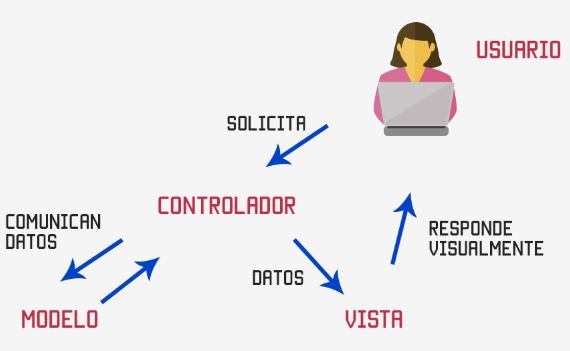
\includegraphics[width=.65\textwidth]{images/marcoteorico/mvc}
		\caption{Imagen que ilustra el modelo Vista-Controlador}
		\label{fig:mvc}
	\end{center}
\end{figure}

MVC desacopla las vistas y los modelos al establecer un protocolo de suscripción / notificación entre ellos. Una vista debe garantizar que su apariencia refleje el estado del modelo. Cada vez que los datos del modelo cambian, el modelo notifica las vistas que dependen de él. En respuesta, cada vista tiene la oportunidad de actualizarse. Este enfoque le permite adjuntar múltiples vistas a un modelo para proporcionar diferentes presentaciones. También puede crear nuevas vistas para un modelo sin reescribirlo.\\

El siguiente diagrama muestra un modelo y tres vistas. (Se omitieron los controladores por simplicidad). El modelo contiene algunos valores de datos, y las vistas que definen una hoja de cálculo, un histograma y un gráfico circular muestran estos datos de varias maneras. El modelo se comunica con sus vistas cuando cambian sus valores, y las vistas se comunican con el modelo para acceder a estos valores. \hyperlink{b20}{[20]} 

\begin{figure}[H]
	\begin{center}
		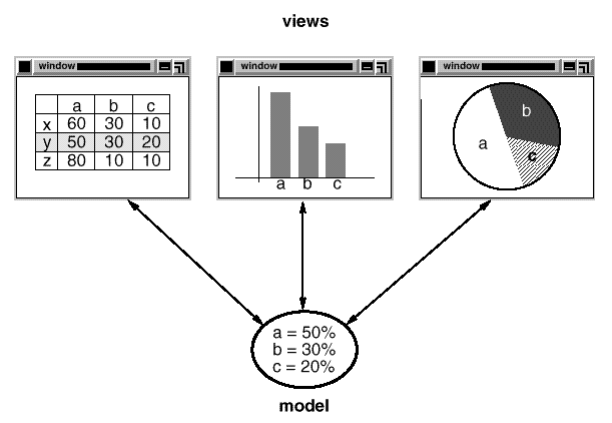
\includegraphics[width=.65\textwidth]{images/marcoteorico/mvc2}
		\caption{Imagen que ilustra un ejemplo de cómo opera el MVC }
		\label{fig:mvc2}
	\end{center}
\end{figure}

\subsection{Framework}

\subsubsection{Definición}
Es un conjunto de clases que encarna un diseño abstracto para soluciones a una familia relacionada de problemas. \hyperlink{b17}{[17]}. 

Conjunto de clases cooperativas que construyen un diseño reutilizable para un tipo específico de software. Un Framework proporciona la arquitectura partiendo el diseño en clases abstractas y definiendo sus responsabilidades y colaboraciones. Un desarrollador realiza una aplicación haciendo subclases y componiendo instancias a partir de las clases definidas por el Framework. \\

Un framework es una aplicación semi-completa, de control invertido, así un Framework difiere de una librería de clases \hyperlink{b17}{[17]}:
\begin{itemize}
	\item En una librería de clases, el control del flujo se encuentra en el código de la aplicación que realiza llamadas a los métodos de la librería de clases.
	\item En un framework, el control del flujo está en código del framework que realiza llamadas al código de la aplicación (control invertido).
\end{itemize}

\subsubsection {Ventajas de un framework}
Como ventajas en la utilización de un framework tenemos las siguientes:

\begin{enumerate}
	\item Minimiza tiempos de desarrollo / acorta el “Time to market”
	\begin{itemize}
	\item Los proyectos de desarrollo ya no tendrán que resolver los múltiples problemas asociados a las aplicaciones web.
	\item  Los frameworks reducen la codificación y sobretodo la puesta en marcha, ya que proporcionan subsistemas que sabemos que ya funcionan. \item  En definitiva, proporcionan código que no se tendrá que mantener ni reescribir.
	\end{itemize}
	\item Reduce los riesgos del desarrollo.
	\begin{itemize}
		\item Con un modelo de programación complejo como el de J2EE, el riesgo de fallos en los proyectos iniciales es alto.
	\end{itemize}
	\item Proporciona una arquitectura consistente entre aplicaciones.
	\begin{itemize}
		\item Al usar frameworks todas las aplicaciones generadas comparten una arquitectura común. Esto hace que sea más fácil de aprender, mantener y soportar.
		\item Cualquier programador que trabaje con un framework no deberá invertir gran parte de su tiempo en buscar las clases necesarias, interconectarlas o descubrir los métodos que contienen. Los frameworks ocultan toda esta complejidad dando un alto nivel de abstracción. 
	\end{itemize}
\end{enumerate}

\newpage

\section{Pruebas}

Con base en los enunciados de la ISTQB (International Software Testing Qualifications Board). \hyperlink{b34}{[34]} Las pruebas de software muestran la presencia de defectos: "todo tipo de software que se desarrolle es susceptible a la presencia de «Bug`s» o defectos y con las pruebas de software se busca reducir al máximo la presencia de estos".\\

También menciona que existen diferentes técnicas de prueba de software, cada una con sus propias fortalezas y debilidades. Cada técnica individual es buena para encontrar tipos particulares de defectos y relativamente pobre para encontrar otros tipos.
En términos generales, hay dos categorías principales, estática y dinámica. Las técnicas cubiertas se resumen en la Figura 2.4.
 
\begin{figure}[H]
	\begin{center}
		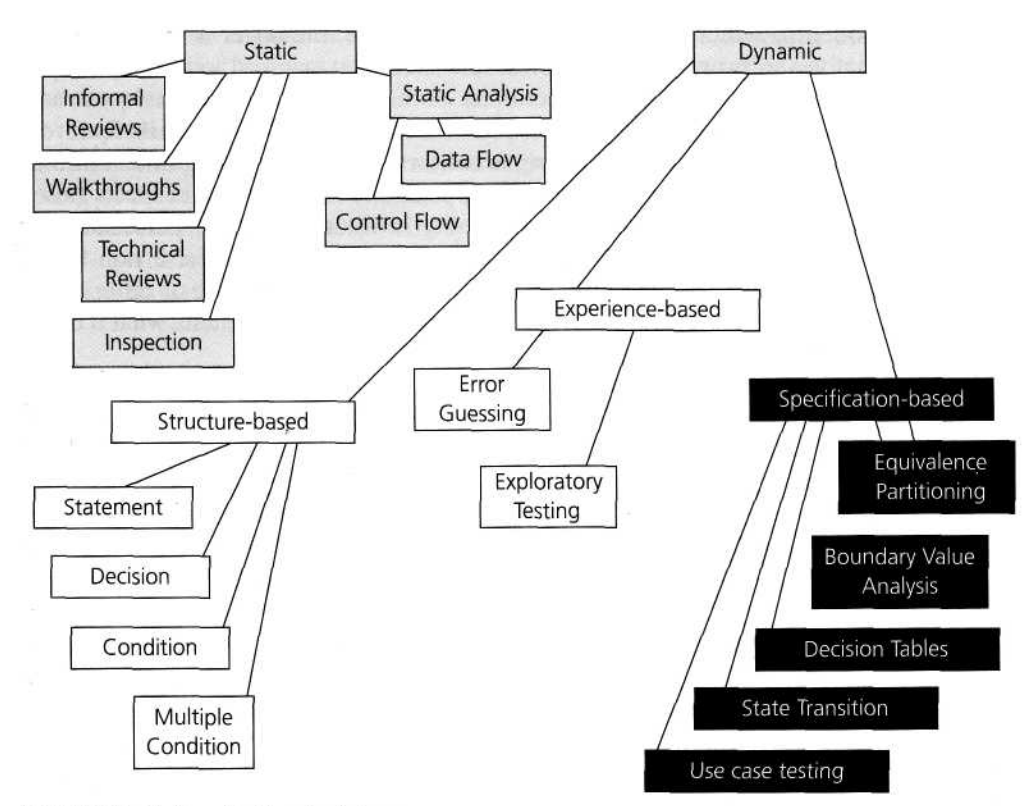
\includegraphics[width=.70\textwidth]{images/marcoteorico/tecnicas}
		\caption{Técnicas de pruebas}
		\label{fig:tecnicas}
	\end{center}
\end{figure}

\subsection{Pruebas Dinámicas}

La ISTQB (International Software Testing Qualifications Board) menciona que la pruebas dinámicas son todas aquellas pruebas que para su realización requieren la ejecución de la aplicación. Las pruebas dinámicas permiten el uso de técnicas de caja negra y caja blanca con mayor amplitud. A continuación se explica su utilidad.
\begin{enumerate}
	\item \textbf {Pruebas de caja negra o basadas en especificación}: Se conocen como técnicas de prueba impulsadas por entrada / salida porque ven el software como un recuadro negro con entradas y salidas, pero no se tiene un conocimiento de cómo se estructura el sistema o componente dentro de la caja. En esencia, está concentrando en lo que hace el software, no en cómo lo hace.
	
		La definición menciona pruebas tanto funcionales como no funcionales.
		\begin{itemize}
			\item \textbf {Pruebas Funcionales}: Se refieren a lo que hace el sistema, sus características o funciones.
			\item \textbf {Pruebas No Funcionales}: Se refieren a examinar qué tan bien el sistema hace algo, en lugar de lo que hace. Los aspectos no funcionales (también conocidos como características de calidad o atributos de calidad) incluyen rendimiento, usabilidad, portabilidad, mantenibilidad, etc. 
		\end{itemize}
	
		Existen cinco técnicas basadas en especificaciones las cuales son:
		\begin{itemize}
			\item \textbf {Clases de equivalencia}: La idea detrás de la técnica es dividir un conjunto de condiciones de prueba en grupos o conjuntos que se pueden considerar iguales. La técnica requiere que solo necesitemos probar una condición de cada partición. Si una condición en una partición funciona o no, asumimos que todas las condiciones en esa partición tendrán el mismo comportamiento.
			\item \textbf {Análisis del valor límite}: Se basa en pruebas en los límites entre particiones. Opera realizado la 'verificación de rango', se tiene que tener en cuenta que tenemos límites válidos (en las particiones válidas) y límites inválidos (en las particiones inválidas).
			\item \textbf {Tablas de decisión}: Proporcionan una forma sistemática de establecer reglas de negocios comerciales complejas. Ayudan a explorar los efectos de combinaciones de diferentes entradas y otros estados de software que deben implementar correctamente las reglas de negocio. Ayudan a la selección sistemática de casos de prueba efectivos, pueden encontrar problemas y ambigüedades en la especificación. Es una técnica que funciona bien junto con la partición de equivalencia. La combinación de condiciones exploradas puede ser combinaciones de particiones de equivalencia.
			\item \textbf {Prueba de transición de estado}: Se utiliza cuando se puede describir algún aspecto del sistema en lo que se llama una "máquina de estados finitos". Esto simplemente significa que el sistema puede estar en un número (finito) de estados diferentes, y las transiciones de un estado a otro están determinadas por las reglas de la 'máquina'.
			\item \textbf {Prueba de caso de uso}:
			La prueba de casos de uso es una técnica que nos ayuda a identificar casos de prueba que ejercitan todo el sistema transacción por transacción de principio a fin. Ivar Jacobson los describe en su libro Ingeniería de software orientada a objetos: un enfoque orientado a casos de uso [Jacobson, 1992] .
		\end{itemize}
	
	\item \textbf {Pruebas de caja blanca}: Las técnicas de prueba basadas en la estructura utilizan la estructura interna del software para derivar casos de prueba. Se denominan comúnmente técnicas de 'caja blanca' o 'caja de cristal' (lo que implica que puede ver el sistema), ya que requieren conocer cómo se implementa el software, es decir, cómo funciona. Por ejemplo, una técnica estructural puede estar relacionada con el ejercicio de bucles en el software.
	
	\item \textbf {Basadas en experiencia}: En las técnicas basadas en la experiencia, el conocimiento, las habilidades y los antecedentes de las personas son los principales contribuyentes a las condiciones y casos de prueba. La experiencia de los técnicos y los empresarios aporta diferentes perspectivas al análisis de prueba y al proceso de diseño ya pueden tener información sobre lo que podría salir mal, lo cual es muy útil para las pruebas.

\end{enumerate}

Dentro de las pruebas dinámicas podemos encontrar distintos niveles de prueba, estos son grupos de actividades que se organizan y gestionan juntas. Cada nivel de prueba es una instancia del proceso de prueba, desde unidades individuales o componentes hasta sistemas completos o, en su caso, sistemas de sistemas.\\

Los niveles de prueba utilizados pueden ser:

\begin{itemize}
	\item \textbf {Prueba de Componente}
	\item \textbf {Prueba de Integración}
	\item \textbf {Prueba de Sistema}
	\item \textbf {Prueba de Aceptación}
\end{itemize}

Los niveles de prueba se caracterizan por los siguientes atributos:

\begin{itemize}
	\item \textbf {Objetivos específicos}
	\item \textbf {Base de prueba, referenciada para derivar casos de prueba}
	\item \textbf {Objeto de prueba (es decir, lo que se está probando)}
	\item \textbf {Defectos y fallas típicas}
\end{itemize}

\subsubsection{Prueba de sistema}

Las pruebas del sistema se centran en el comportamiento y las capacidades de un sistema o producto completo, a menudo considerando las tareas de extremo a extremo que el sistema puede realizar y los comportamientos no funcionales que exhibe mientras realiza esas tareas. Este nivel de pruebas tiene como objetivo: la reducción de riesgos, verificar si los comportamientos funcionales y no funcionales del sistema son los diseñados y especificados, alidar que el sistema está completo y funcionará como se esperaba, generar confianza en la calidad del sistema en su conjunto, encontrar defectos y Evitar que los defectos escapen a niveles de prueba o producción más altos.

\begin{table}[H]
	\centering
	\begin{tabular}{|p{3.5cm}|p{13cm}|}
		\hline
		\centering \textbf{Base de prueba} & \begin{itemize}
			\item Especificaciones de requisitos del sistema y software (funcionales y no funcionales)
			\item Informes de análisis de riesgos.
			\item Casos de uso
			\item Epicas e historias de usuarios.
			\item Modelos de comportamiento del sistema.
			\item Diagramas de estado.
			\item Sistema y manuales de usuario.
		\end{itemize}
		  \\
		\hline
		\centering \textbf{Objeto de prueba} & \begin{itemize}
			\item Aplicaciones (de escritorio o móviles)
			\item Sistemas de hardware / software
		\end{itemize}  \\
		\hline
	\end{tabular}
\end{table}


\subsection{Pruebas Estáticas}

Las pruebas estáticas encuentran defectos en los productos de trabajo directamente en lugar de identificar fallas causadas por defectos cuando se ejecuta el software.  En comparación con las pruebas dinámicas, los defectos típicos que son más fáciles y baratos de encontrar y reparar mediante pruebas estáticas incluyen:
\begin{itemize}
	\item \textbf {Defectos de requisitos} (inconsistencias, ambigüedades, contradicciones, omisiones, imprecisiones y redundancias)
	\item \textbf {Defectos de diseño} (algoritmos ineficientes o estructuras de bases de datos, alto acoplamiento, baja cohesión)
	\item \textbf {Defectos de codificación} (variables con valores indefinidos, variables que se declaran pero nunca se usan, código inalcanzable, código duplicado)
	\item \textbf {Desviaciones de los estándares} (falta de adherencia a los estándares de codificación)
\end{itemize}

La mayoría de los tipos de defectos de mantenimiento solo se pueden encontrar mediante pruebas estáticas (por ejemplo, modularización inadecuada, mala reutilización de componentes, código que es difícil de analizar y modificar sin introducir nuevos defectos).A diferencia de las pruebas dinámicas, las pruebas estáticas encuentran defectos en lugar de fallas.\\

\subsubsection {Defectos de Codificación}

Para el análisis estático hay muchas herramientas, y la mayoría de ellas se centran en el código de software. Las herramientas pueden mostrar no solo atributos estructurales (métricas de código), como la profundidad de anidamiento o el número ciclomático y verificar los estándares de codificación, sino también representaciones gráficas del flujo de control, las relaciones de datos y el número de rutas distintas de una línea de código a otra. Incluso el compilador puede considerarse una herramienta de análisis estático, ya que crea una tabla de símbolos, señala el uso incorrecto y comprueba el incumplimiento de las convenciones del lenguaje de codificación (sintaxis).

Estos problemas se pueden encontrar utilizando herramientas de análisis estático para detectarlos. 

\begin{itemize}
	\item \textbf {Estándares de codificación:} Verificar la adherencia a los estándares de codificación es la más conocida de todas las características. La primera acción a tomar es definir o adoptar un estándar de codificación. Por lo general, un estándar de codificación consta de un conjunto de reglas de programación (p. Ej., 'Verifique siempre los límites de una matriz al copiar en esa matriz'), convenciones de nomenclatura (p. Ej., 'Las clases deben comenzar con C mayúscula) y especificaciones de diseño (p. Ej.,' Sangría 4 espacios ' ) Se recomienda que se adopten las normas existentes. 
	\item \textbf {Métricas de código:} Cuando se realiza un análisis de código estático, generalmente se calcula la información sobre los atributos estructurales del código, como la frecuencia de comentarios, la profundidad de anidación, el número ciclomático y el número de líneas de código.
	\item \textbf {Estructura de código:} 
	 Hay varios aspectos de la estructura del código a considerar:
	\begin{itemize}
		\item Estructura de flujo de control: La estructura de flujo de control aborda la secuencia en la que se ejecutan las instrucciones.
		\item Estructura de flujo de datos: Sigue el rastro de un elemento de datos a medida que el código accede y lo modifica.
		\item Estructura de datos: La estructura de datos se refiere a la organización de los datos en sí, independientemente del programa.
	\end{itemize}
\end{itemize}

\subsubsection{SonarQube }

Es una plataforma de código abierto desarrollada por SonarSource para la inspección continua de la calidad del código para realizar revisiones automáticas con análisis estático del código para detectar errores de código y vulnerabilidades de seguridad en más de 20 lenguajes de programación . Sonarqube ofrece informes sobre código duplicado , estándares de codificación , pruebas unitarias , cobertura de código , la complejidad del código , comentarios, errores y vulnerabilidades de seguridad.\hyperlink{b36}{[36]}\\

SonarQube puede registrar el historial de métricas y proporciona gráficos de evolución. SonarQube proporciona análisis e integración totalmente automatizados con Maven , Ant , Gradle , MSBuild y herramientas de integración continua ( Atlassian Bamboo , Jenkins , Hudson , etc.).\hyperlink{b37}{[37]}\\

Esta herramienta nos provee la covertura de los 7 pilares dentro de la calidad del código:

\begin{itemize}
	\item Arquitectura y Diseño.
	\item Comentarios.
	\item Reglas de Código.
	\item Errores potenciales.
	\item Complejidad.
	\item Tests de Unidad.
	\item Duplicaciones.
\end{itemize}






%=========================================================
%=========================================================
\chapter{Estado del Arte} \label{cap:tres}

	Es común que dentro del área de la ingeniería de software, se confundan los términos: ''Caso de uso'' y ''Diagrama de caso de uso'', sin embargo es importante resaltar las diferencias para comprender el objetivo principal del proyecto terminal.
	
	\begin{quote}
		\small Un caso de uso narra una historia detallada sobre cómo interactúa un usuario final (con cierto número de roles posibles) con el sistema en circunstancias específicas. La historia puede ser un texto narrativo, un lineamiento de tareas o interacciones, una descripción basada en un formato o una representación diagramática de casos de uso. Sin importar su forma, un caso de uso ilustra el software o sistema desde el punto de vista del usuario final \hyperlink{b07}{[7]}. 
	\end{quote}
	 	
	En otras palabras, un caso de uso es aquel que describe en forma de secuencia de acciones o pasos la interacción entre un actor y el sistema, en cambio, un diagrama de casos de uso es una representación visual simple de las interacciones del sistema con el mundo exterior, el modelo de un grafo con dos tipos de nodos (Actor y caso de uso), el cual ilustra gráficamente el comportamiento del caso de uso. Un diagrama de casos de uso no describe la interacción detallada del sistema con los actores ni reemplaza o sustituye el concepto de caso de uso.\\
	
	Ahora bien, en la red hay una gran variedad de sistemas que permiten la generación de \textbf {diagramas de casos de uso en UML} ,a partir de distintas técnicas, sin embargo no hay herramientas comerciales o gratuitas que posibiliten la generación del documento con las especificaciones y la gestión de sus componentes, tal como lo pretende el presente trabajo terminal.
	
%	\newline
    \newpage
%---------------------------------------------------------
\section{Antecedentes}

\subsection{UCD-Generator - Una aplicación LESSA para el diseño de casos de uso}

Las herramientas CASE convencionales requieren una comprensión completa del negocio, una gran cantidad de tiempo y esfuerzos adicionales por parte del analista del sistema durante el proceso de creación, organización, etiquetado y finalización de los diagramas de casos de uso. Es por esto que se diseñó un sistema que proporciona una manera rápida y confiable de generar diagramas de casos de uso para ahorrar tiempo y presupuesto tanto para el usuario como para el analista del sistema.

\subsubsection{Objetivo}
Este sistema presenta un enfoque basado en el procesamiento del lenguaje natural LESSA (Language Engineering System for semantic analysis) que se utiliza para comprender automáticamente el texto en lenguaje natural y extraer la información requerida. Esta información se utiliza para dibujar los diagramas de casos de uso. El usuario escribe sus preferencias basadas en la interfaz en inglés, en unos pocos párrafos y el sistema diseñado tiene una capacidad notable para analizar el script dado. Después del análisis compuesto y la extracción de información asociada, el sistema diseñado en realidad dibuja los diagramas de casos de uso \hyperlink{b08}{[8]}.  

\subsection{Generación automatizada de diagramas de casos de uso a partir de requerimientos de usuarios}

Con el estado actual de la tecnología de procesamiento de lenguaje natural (PNL), muchos investigadores han demostrado que automatizar el proceso de análisis de requisitos es posible, lo que ahorra una cantidad significativa de tiempo invertido por los analistas. Se han desarrollado numerosas herramientas semiautomáticas que ayudan al analista en este proceso. Sin embargo, una técnica comúnmente utilizada para usar la gramática en el texto obtenido como la base para identificar información útil, ha estado enfrentando problemas de escalabilidad debido a que el formato textual de los requisitos consiste en lenguaje natural no estructurado (NL). 

\subsubsection{Objetivo}
Este proyecto utiliza una técnica probabilística para identificar actores y casos de uso. El resultado prometedor demuestra que las mejoras adicionales de este enfoque pueden automatizar completamente la fase de análisis, propone una metodología para la asistencia automática de análisis de requisitos a los analistas de software mediante la extracción de un diagrama de caso de uso del documento de requisitos del usuario.
Este proyecto ha intentado con éxito extraer actores y usar casos utilizando un modelo de clasificación probabilística junto con una asistencia mínima de enfoque basado en reglas. Los casos de uso son nítidos y consistentes independientemente del tamaño del texto de los requisitos. Debido al pequeño tamaño de los datos utilizados, el rendimiento no se ha logrado precisar. Sin embargo, se pueden utilizar mejores modelos de clasificación con un conjunto de datos más grande que incluya otros dominios de software para mejorar los resultados. El desafío restante aquí se relaciona con abordar los requisitos no funcionales y también para incorporar funciones de inclusión y extensión al diagrama de casos de uso. Un gráfico bien diseñado \hyperlink{b09}{[9]}.
%=========================================================
\chapter{Análisis de mercado} \label{cap:cuatro}

En este apartado se demuestra la viabilidad comercial del trabajo terminal TESSERACT en México, así mismo se realiza un estudio en donde se determina el campo en donde un sistema con las características del generador de documento de casos de uso podría generar un mayor impacto y aceptación por parte de los equipos de desarrollo de software. Cabe resaltar que TESSERACT no pretende ser comercializado por el momento.

%---------------------------------------------------------
\section{Situación actual  y evolución del mercado}

El software es un elemento consustancial a la economía moderna, es uno de los sectores tecnológicos más competitivos, se usa en en una gran cantidad de productos manufacturados y servicios, por lo que  la elaboración de programas de cómputo figura en casi todas las industrias y es, de hecho, factor de éxito de todos los sectores de la economía. Esta industra ha tenido una evolución constante en lo que se refiere a las metodologías o bien, las formas en las cuales se realiza la planeación para el diseño del software, básicamente con el objetivo de mejorar, optimizar procesos y ofrecer una mejor calidad. \hyperlink{b22}{[22]}.\\

En el campo del desarrollo de software, existen dos grupos de metodologías, las denominadas tradicionales (formales) y las ágiles. Las primeras son un tanto rígidas, exigen una documentación exhaustiva y se centran en cumplir con el plan del proyecto definido totalmente en la fase inicial del desarrollo del mismo; mientras que la segunda enfátiza el esfuerzo en la capacidad de respuesta a los cambios, las habilidades del equipo y mantener una buena relación con el usuario. La metodología que sea seleccionada, debe ser adaptada al contexto del proyecto, teniendo en cuenta los recursos técnicos y humanos; tiempo de desarrollo y tipo de sistema. \hyperlink{b24}{[24]}.\\

Dean Leffingwell, autor de Scaling Software Agility, menciona que los Casos de Uso son una herramienta valiosa para modelar requerimientos en metodologías Lean/Ágiles de gran envergadura, si embargo, no es común encontrar casos de uso en los proyectos ágiles (especialmente en XP y Scrum), en donde se suele utilizar historias de usuario para recolectar los requerimientos \hyperlink{b12}{[12]}.\\

Ahora bien, de acuerdo a la teoría expuesta, TESSERACT al ser una herramienta que asiste a la generación del documento de casos de uso, se convierte en un instrumento que puede contribuir en cualquier metodología, ya sea formal o ágil, sin embargo el beneficio e impacto incrementa cuando se utiliza en la construcción de sistemas con metodologias formales y de gran escala, los casos de uso son una herramienta muy poderosa para explorar las interacciones entre los usuarios, los sistemas, y los sub-sistemas. Más aún, la técnica de casos de uso es la mejor forma para identificar todos los escenarios alternativos que se nos aparecen, fundamentales para asegurar la calidad de los sistemas. En los desarrollos ágiles, los casos de uso no reemplazan a las historias de usuario pero pueden resultar sumamente útiles para analizar, elaborar y comprender el funcionamiento deseado de sistemas complejos.

\subsection{Industria Mexicana del Software}

Para conocer el nivel de oportunidad que tiene TESSERACT dentro de la industria en México, es importante conocer de manera cuantitativa cual es el perfil de las empresas desarrolladoras de software en México.\\

\textbf{Localización Geográfica de las Empresas Participantes}\\
 
Las empresas participantes en el estudio se localizan en 11 de los 32 estados de la República Mexicana, presentando la siguiente distribución: 2.9\% Chihuahua, 1.5\%  en Coahuila, 44.1\%  en la Ciudad de México, 11.8\%  en Durango, 2.9\%  en el Estado de México, 1.5\%  en Guanajuato, 2.9\%  en Jalisco, 2.9\%  en Michoacán, 2.9\%  en Morelos, 23.5\%  en Nuevo León y 2.9\%  en Querétaro. Esta concentración es similar a la de otros estudios realizados para este sector en México.\hyperlink{b13}{[13]}\\

\textbf{Número de Empresas Desarrolladoras de Software en México}\\

La respuesta a esta pregunta no tiene una cifra exacta. De acuerdo con estimaciones realizadas por la empresa denominada ``ESANE consultores" sobre el número total de empleados y empresas de la Industria del Software en México, el número aproximado de empresas de la industria mexicana del software podría ser del orden de 1,500 empresas.\hyperlink{b13}{[13]}.\\
 
\textbf{Tamaño de las Empresas}\\

El estudio revela que el 85.29\% de las empresas del sector de la Industria Mexicana del Software son de tamaño micro (54.41\%) y pequeño (30.88\%), el 5.8\% mediana, y tan sólo el 8.82\% son de tamaño grande (con un número de empleados mayor a 100) \hyperlink{b13}{[13]}.\\

Las oportunidades que se tienen de posicionar TESSERACT en el mercado son amplias, la industria del software muestra un constante crecimiento y en México hay posibilidades de colocar nuestra herramienta en diversos sectores para contribuir en el desarrollo y construcción de software. 
%=========================================================


\chapter{Estimación de tiempo y costo} \label{cap:cinco}

\section{Puntos de función}

Es una técnica de estimación de software desarrollada originalmente por Allan Albrecht en 1979 mientras trabajaba para IBM, quien definió conceptos para medir el software a partir de valoraciones de funcionalidades entregadas al usuario y no a partir de aspectos técnicos, con la intención de producir valoraciones independientes de la tecnología y fases del ciclo de vida utilizado.

El trabajo de Albrecht fue continuado por el grupo internacional de usuarios de puntos de función, quienes plasmaron sus conceptos en el método IFPUG-FPA, el cual realiza las valoraciones a partir de la funcionalidad del sistema, primero clasificándolas, luego asignando una complejidad y ponderación a cada una según unas tablas predefinidas, determinando así el valor de puntos de función.

Sumando los puntos de todas las funcionalidades se obtiene la valoración de todo el proyecto y finalmente se puede aplicar un factor de ajuste, que puede depender de características generales del sistema como por ejemplo requerimientos no funcionales como el rendimiento, reusabilidad, facilidad de instalación y operación entre otros aspectos.

Los puntos de función permiten traducir el tamaño de funcionalidades de software a un número, a través de la suma ponderadas de las características que este tiene. Una vez que tenemos los puntos de función, podemos traducirlos en horas hombre o días de trabajo, según factor de conversión que dependería de mediciones históricas de nuestra productividad. Con las horas hombre, podemos determinar el costo y presupuesto de los proyectos. \hyperlink{b12}{[12]}.

\newpage

Desarrollaremos la medición en dos pasos, primero determinaremos los componentes funcionales del presupuesto de desarrollo de software, a partir del análisis de requerimientos realizado anteriormente. Seguidamente, realizaremos el cálculo de los puntos de función, con lo cual obtendremos una medida del tamaño del proyecto.\\

Para determinar los componentes funcionales, debemos determinar tanto las transacciones de negocio como los componentes de datos, siguiendo el método de análisis de puntos de función.  Las transacciones de negocio que podemos desglosar a partir de los requerimientos de software son las siguientes.

\begin{table}[H]
	\centering
	\begin{tabular}{|p{4cm}|p{4cm}|}
		\hline
		\rowcolor{black} \textcolor{white} {\textbf{Tipo de Caso de uso}} & \textcolor{white}{\textbf{Cantidad}} \\ \hline
		Gestionar & 13  \\
		\hline
		Registrar & 18  \\
		\hline
		Modificar o Editar & 15  \\
		\hline
		Eliminar & 17  \\
		\hline
		Buscar & 9  \\
		\hline
	\end{tabular}
\end{table}

Seguidamente, clasificamos las transacciones de negocio, que pueden ser de 3 tipos: Entradas, salidas y consultas. 

\begin{itemize}
\item Entradas: Registrar modificar y eliminar
\item Salida: Gestionar
\item Consultas: Buscar
\item Archivo lógico interno: Tablas en Base de datos

\end{itemize}

Adicionalmente, debemos asignar un nivel de complejidad alto, medio o bajo a cada uno con base en la siguiente tabla.

	\begin{table}[H]
	\centering
	\begin{tabular}{|p{3cm}|p{1cm}|p{1cm}|p{1cm}|}
		\hline
		\rowcolor{black} \textcolor{white} {\textbf{Tipo}} & \textcolor{white}{\textbf{Baja}} & \textcolor{white}{\textbf{Media}} & \textcolor{white}{\textbf{Alta}} \\ \hline
		Entrada  externa (EI) & 3PF & 4PF & 6PF  \\
		\hline
		Salida  externa (EO) & 4PF & 5PF & 7PF  \\
		\hline
		Consulta  externa (EQ) & 3PF & 4PF & 6PF  \\
		\hline
		Archivo lógico interno (ILF) & 7PF & 10PF & 15PF  \\
		\hline
		Archivo de interfaz externo (ILF) & 5PF & 7PF & 10PF  \\
		\hline
	\end{tabular}
\end{table}

Los niveles de complejidad dependen de factores como por ejemplo el número de campos no repetidos, número de archivos a ser leídos, creados o actualizados, número de sub grupos de datos o formatos de registros, entre otros.

Al clasificar las transacciones de negocio y asignar los niveles de complejidad se llegó a la conclusión que para el desarrollo de TESSERACT, la complejidad en todos sus niveles es \textbf {MEDIA}

Al determinar los puntos de función tenemos una medida de la magnitud del tamaño del software y del esfuerzo que se requiere para desarrollarlo.

\begin{table}[H]
	\centering
	\begin{tabular}{|p{4cm}|p{3cm}|p{3cm}|p{3cm}|}
		\hline
		\rowcolor{black} \textcolor{white} {\textbf{Tipo de Caso de uso}} & \textcolor{white}{\textbf{Cantidad}} & \textcolor{white}{\textbf{Complejidad}} & \textcolor{white}{\textbf{Total PF}} \\ 
		\hline
		Gestionar & 13  &  5 &  65  \\
		\hline
		Registrar & 18 &  4 &  72 \\
		\hline
		Modificar o Editar & 15 &  4 &  60  \\
		\hline
		Eliminar & 17 &  4 &  68  \\
		\hline
		Buscar & 9 &  4 &  36 \\
		\hline
		Tablas en BD & 65 &  10 &  650 \\
		\hline
	\end{tabular}
\end{table}

\textbf {MAGNITUD ESTIMADA:} 951 PF\\

\begin{table}[H]
	\centering
	\begin{tabular}{|p{5cm}|p{3cm}|p{3cm}|}
		\hline
		\rowcolor{black} \textcolor{white} {\textbf{Lenguaje}} & \textcolor{white}{\textbf{Horas PF Promedio}} & \textcolor{white}{\textbf{Lineas de código por PF}} \\ \hline
		Lenguajes de 4ta generación & 8  & 20 \\
		\hline
	\end{tabular}
\end{table}

\textbf {HORAS HOMBRE:} 7608 hrs para que una persona termine el sistema.\\


Ahora bien para estimar el tiempo se tienen los siguientes datos:

\begin{table}[H]
	\centering
	\begin{tabular}{|p{4cm}|p{4cm}|}
		\hline
		\rowcolor{black} \textcolor{white} {\textbf{Concepto}} & \textcolor{white}{\textbf{Tiempo}} \\ \hline
		Desarrolladores & 4  \\
		\hline
		Horas de trabajo al día & 8  \\
		\hline
		Días al mes de trabajo & 24  \\
		\hline
		Horas de trabajo x desarrollador & 1902  \\
		\hline
		Dias de trabajo x desarrollador & 237  \\
		\hline
		Meses de trabajo  & 10  \\
		\hline
	\end{tabular}
\end{table}

\textbf {TIEMPO ESTIMADO:} 10 meses para desarrollar el software, con un trabajo de lunes a sábado, 8 hrs diarias con 4 desarrolladores.\\

Para estimar el costo del proyecto se tiene la siguiente información:

\textbf {TIEMPO ESTIMADO:} 10 MESES \\
\textbf {DESARROLLADORES:} 4 DESARROLLADORES\\

\begin{table}[H]
	\centering
	\begin{tabular}{|p{4cm}|p{4cm}|p{4cm}|}
		\hline
		\rowcolor{black} \textcolor{white} {\textbf{Concepto}} & \textcolor{white}{\textbf{Cantidad}} & \textcolor{white}{\textbf{Total}} \\ \hline
		Sueldo Mensual de un desarrollador & \$18,000 & \$720,000   \\
		\hline
		Consumo de luz por mes & \$125  & \$1250 \\
		\hline
		Consumo de agua por mes & \$50  & \$500  \\
		\hline
		Otros costos del proyectopor mes & \$850  & \$8500  \\
		\hline
	\end{tabular}
\end{table}

Datos salariales promedios obtenidos de https://www.indeed.com.mx/salaries/Desarrollador/a-java-Salaries

\textbf {COSTO TOTAL ESTIMADO:} \$730,250  \\

%=========================================================
%\chapter{Análisis de Riesgos} \label{cap:seis}
%=========================================================
\chapter{Metodología} \label{cap:siete}

En este capítulo se describen las actividades realizadas durante cada uno de los sprints planteados para la entrega del trabajo terminal.\\

De acuerdo a las necesidades del proyecto, se determinó trabajar con base en la metodología scrum empleando específicamente el uso de sprints.\\

El núcleo central de la metodología de trabajo ‘scrum’ es el ‘sprint’. Se trata de un miniproyecto de no más de un mes (ciclos de ejecución muy cortos -entre una y cuatro semanas), cuyo objetivo es conseguir un incremento de valor en el producto que estamos construyendo. Todo ‘sprint’ cuenta con una definición y una planificación que ayudará a lograr las metas marcadas. \hyperlink{b21}{[21]}\\ 

Scrum, que se emplea cada vez con más frecuencia para desarrollar productos y servicios digitales, es un marco de trabajo donde los miembros de un equipo colaboran en la construcción de un producto de manera que sea valioso desde sus primeras etapas. Para lograr esta entrega de valor tan rápida y continua, los equipos ‘scrum’ trabajan en ciclos de ejecución muy cortos -entre una y cuatro semanas- que se denominan ‘sprints’ y tienen un objetivo muy claro. \hyperlink{b21}{[21]}\\ 

El primer paso para alcanzar este objetivo -o hito del proyecto- es la reunión de planificación, una sesión en la que debe participar todo el equipo ‘scrum’ y que supone el pistoletazo de salida del ‘sprint’. Esta reunión se divide en dos partes que tratan de dar respuesta a dos preguntas fundamentales: ¿Qué se va a entregar? y ¿cómo se va a realizar el trabajo?, donde cada miembro inspecciona el trabajo de los otros para poder hacer las adaptaciones necesarias, comunica cuales son los confictos en los que se encuentra, actualiza el estado de la lista de tareas de la iteración (Sprint Backlog) y los gráficos de trabajo pendiente (Burndown charts). \hyperlink{b22}{[22]}\\ 

\section{Sprint 0: Configuración del ambiente de trabajo}
\subsection{Selección de herramientas}

A continuación se detallan las herramientas consideradas para el desarrollo del proyecto, así como la justificación de las alternativas seleccionadas.\\

En primer lugar se describe en el cuadro \ref{tbl:compotex} las herramientas de composición de textos seleccionadas que pueden coadyuvarnos en la edición de los documentos entregables.

\begin{table}[H]
	\centering
	\begin{tabular}{|p{3cm}|p{12cm}|}
		\hline
		 \rowcolor{black} \textcolor{white}{\textbf{Herramienta}} & \textcolor{white}{\textbf{Características}}  \\ \hline
		Latex & Es un sistema de software libre y de composición tipográfica de alta calidad, esta herramienta incluye características diseñadas para la producción de la documentación técnica en donde se establecen las características del proyecto.\hyperlink{b54}{[54]}\\
		\hline
		Word & Es un programa informático orientado al procesamiento de textos. Fue creado por la empresa Microsoft, y viene integrado de manera predeterminada en el paquete ofimático denominado Microsoft Office. \hyperlink{b53}{[53]}\\
		\hline
		Google Docs & Procesador de texto es una aplicación informática que permite crear y editar documentos de texto en una computadora. Se trata de un software de múltiples funcionalidades para la redacción, con diferentes tipografías, tamaños de letra, colores, tipos de párrafos, efectos artísticos y otras opciones. \hyperlink{b55}{[55]}\\
		\hline
	\end{tabular}
\caption{Cuadro de características de las herramientas para el sistema de composición de textos.}
\label{tbl:compotex}
\end{table}

\textbf {HERRAMIENTA SELECCIONADA: LATEX}\\

\textbf {JUSTIFICACIÓN:} Para la elaboración de nuestros entregables, Latex nos facilita la generación de todo tipo de índices, listados de bibliografía citada, permite centrarnos en el contenido, no en la forma. Los documentos tendrán un contenido extenso por lo que necesitamos un reducido tiempo de generación del documento, Latex es rápido, limpio y seguro, sin olvidar que al realizar todos los cambios de formato no se altera el estilo a comparación de Word.\\
\newpage
En el cuadro \ref{tbl:lenguaje} se exponen las características de los lenguajes de programación para elegir el que mejor se adapta a nuestro proyecto.

\begin{table}[H]
	\centering
	\begin{tabular}{|p{3cm}|p{12cm}|}
		\hline
		\rowcolor{black}  \textcolor{white}{\textbf{Herramienta}} & \textcolor{white}{\textbf{Características}}  \\ \hline
		Java &  Es una tecnología que se usa para el desarrollo de aplicaciones que convierten a la Web en un elemento más interesante y útil. Java es la base para prácticamente todos los tipos de aplicaciones de red, además del estándar global para desarrollar y distribuir aplicaciones móviles y embebidas, juegos, contenido basado en web y software de empresa.\hyperlink{b56}{[56]} \\
		\hline
		C Sharp & C\# es un lenguaje de tipos y orientado a objetos que permite a los desarrolladores crear una gran variedad de aplicaciones seguras y sólidas que se ejecutan en .NET Framework. Puede usar C\# para crear aplicaciones cliente de Windows, servicios web XML, componentes distribuidos, aplicaciones cliente-servidor y aplicaciones de base de datos.\hyperlink{b57}{[57]} \\
		\hline
		Python & Python es un lenguaje de programación web de alto nivel basado en un código compacto, pero con una sintaxis fácil de entender. Es un lenguaje de programación multiparadigma. Esto significa que más que forzar a los programadores a adoptar un estilo particular de programación, permite varios estilos: programación orientada a objetos, programación imperativa y programación funcional. Otros paradigmas están soportados mediante el uso de extensiones.\hyperlink{b58}{[58]} \\
		\hline

	\end{tabular}
\caption{Cuadro de características de las herramientas de leguajes de programación.}
\label{tbl:lenguaje}
\end{table}

\textbf {HERRAMIENTA SELECCIONADA: JAVA}\\

\textbf {JUSTIFICACIÓN:} La idea principal de TESSERACT es que opere como una plataforma Web, java al ser un lenguaje multiplataforma nos permite construir un producto con las características deseadas. C\# no es un lenguaje multiplataforma y Phyton no nos proporciona muchos recursos. Otras de las ventajas que tiene java son sus librerias estandar, la facilidad de programación y su paradigma orientado a objetos. 
\newpage
Después de haber seleccionado el lenguaje de programación hay que adaptar el uso de un framework para del desarrollo. En el cuadro \ref{tbl:frame} se exponen las características de los frameworks para elegir la que mejor se adapta a nuestro proyecto.

\begin{table}[H]
	\centering
	\begin{tabular}{|p{3cm}|p{12cm}|}
		\hline
		\rowcolor{black} \textcolor{white} {\textbf{Herramienta}} & \textcolor{white}{\textbf{Características}}  \\ \hline
		Struts 2 & Apache Struts 2 es un marco de aplicación web de código abierto para desarrollar aplicaciones web Java EE . Utiliza y amplía la API de Java Servlet para alentar a los desarrolladores a adoptar una arquitectura modelo-vista-controlador (MVC). El marco de trabajo WebWork surgió de Apache Struts con el objetivo de ofrecer mejoras y refinamientos al tiempo que conserva la misma arquitectura general del marco original de Struts. \hyperlink{b59}{[59]} \\
		\hline
		Spring & Spring es un framework para el desarrollo de aplicaciones y contenedor de inversión de control, de código abierto para la plataforma Java. Nos ofrece la posibilidad de crear código de alto rendimiento, liviano y reutilizable. Ya que su finalidad es estandarizar, agilizar, manejar y resolver los problemas que puedan ir surgiendo en el trayecto de la programación. \hyperlink{b59}{[59]} \\
		\hline
		Server Faces & Java Server Faces es un framework MVC (Modelo-Vista-Controlador) basado en el API de Servlets que proporciona un conjunto de componentes en forma de etiquetas definidas en páginas XHTML mediante el framework Facelets. Facelets se define en la especificación 2 de JSF como un elemento fundamental de JSF que proporciona características de plantillas y de creación de componentes compuestos. Antes de la especificación actual se utilizaba JSP para componer las páginas JSF. \hyperlink{b60}{[60]}\\
		\hline
	\end{tabular}
\caption{Cuadro de características de los frameworks estudiados.}
\label{tbl:frame}
\end{table}

\textbf {HERRAMIENTA SELECCIONADA: STRUTS 2}\\

\textbf {JUSTIFICACIÓN:}
Al usar un framework y seguir su convención, estamos programando de una manera aceptada, ya que esta es la idea que constituye la base de los patrones de diseño.  A pear de que como lo vimos en la comparativa, struts no es el único framework MVC existente en J2EE si es el más extendido y por lo tanto, usando Struts dispondremos de una gran cantidad de recursos: documentación (tutoriales, artículos, libros). El código para configurar repeticiones ya no es necesario porque los interceptores se ocupan de ello . La aportación principal de JSF no es MVC sino los componentes gráficos de usuario (GUI) de ``alto nivel" para la web. Por último con base en la experiencia obtenido Struts es el lenguaje más estudiado.\\

\newpage

 En el cuadro \ref{tbl:sgbd} se exponen las características de los gestores de bases de datos para elegir el que mejor se adapte a nuestro proyecto.

\begin{table}[H]
	\centering
	\begin{tabular}{|p{3cm}|p{12cm}|}
		\hline
		\rowcolor{black} \textcolor{white} {\textbf{Herramienta}} & \textcolor{white}{\textbf{Características}}  \\ \hline
		MySQL & Es el sistema gestor de bases de datos relacional por excelencia.
		Es un SGBD multihilo y multiusuario utilizado en la gran parte de las páginas web actuales. Además es el más usado en aplicaciones creadas como software libre. 
		Las principales ventajas de este Sistema Gestor de Bases de datos son: Facilidad de uso y gran rendimiento, facilidad para instalar y configurar, soporte multiplataforma y soporte SSL. \hyperlink{b61}{[61]}\\
		\hline
		MariaDB & Este SGBD es una derivación de MySQL que cuenta con la mayoría de características de este e incluye varias extensiones. Entre las principales características de este Sistema Gestor de Bases de datos se encuentran: Aumento de motores de almacenamiento, gran escalabilidad, seguridad y rapidez en transacciones, extensiones y nuevas características relacionadas con su aplicación para Bases de datos NoSQL. \hyperlink{b61}{[61]} \\
		\hline
		PostgreSQL & Sus principales características son: control de Concurrencias multiversión (MVCC), flexibilidad en cuanto a lenguajes de programación multiplataforma, pispone de una herramienta (pgAdmin, https://www.pgadmin.org/) muy fácil e intuitiva para la administración de las bases de datos. Robustez, Eficiencia y Estabilidad.
		La principal desventaja es la lentitud para la administración de bases de datos pequeñas ya que está optimizado para gestionar grandes volúmenes de datos. \hyperlink{b61}{[61]}\\
		\hline
	\end{tabular}
	\caption{Cuadro de características de los SGBD (Sistema Gestor de Bases de Datos) estudiados.}
	\label{tbl:sgbd}
\end{table}

\textbf {HERRAMIENTA SELECCIONADA: MySQL}\\

\textbf {JUSTIFICACIÓN:}
MySQL es el gestor más utilizado en los proyectos escolares, razón por la cual es la herramienta con la que más experiencia se cuenta, sin olvidar que la velocidad al realizar las operaciones es alta, es uno de los gestores con mejor rendimiento, tiene un bajo consumo de recursos, es fácil de configurar e instalar. Soporta gran variedad de Sistemas Operativos y se adapta perfectamente a las necesidades del proyecto.
\newpage
\section{Sprint 1: Gestión de colaboradores}

\subsection{Iniciar sesión}
\subsubsection {Análisis}
Se requiere un proceso mediante el cual se controle el acceso individual al sistema mediante la identificación de usuario utilizando credenciales provistas por el registro de personal.\\

\subsection{Gestionar colaborador}
El actor puede visualizar aquellas personas de la organización que se encuentran involucradas en uno o más proyectos, del  mismo modo el actor puede realizar diferentes acciones, como un nuevo registro o consultar, modificar y eliminar personas previamente registradas.

\subsubsection {Análisis}
Es importante tener un mecanismo de control sobre aquellas entidades humanas que participan en las activades, toma de desiciones y otras funciones dentro de un proyecto de software. Estas personas pueden estar involucradas en uno o más proyectos.
\bigskip
El administrador, tiene la facultad y poder de:\\

\textbf {Registrar colaborador:} Para el registro fué de suma importancia establecer los datos de entrada más relevantes para el sistema, esto con el fin de no saturar la base de datos.\\

La información solicitada para el registro de personal es la siguiente:

\begin{itemize}
	\item \textbf{CURP:} Con el fin de tener unicidad de registros en la base de datos.
	\item \textbf{Nombre, Primer Apellido, Segundo Apellido:} Con el fin de identificar a las personas.
	\item \textbf{Correo electrónico:} Para utilizarse como nombre de usuario en el inicio de sesión.
	\item \textbf{Contraseña:} Con el fin de tener una autenticación segura y comprobada en el sistema.
\end{itemize}

Una vez que se realiza el registro de una persona de manera exitosa, esta podrá participar en algún proyecto.\\

\textbf {Modificar colaborador:} Dentro del sistema existe la posibilidad de que los datos de una persona previamente registrada sean modificados, a excepción de la CURP.

\textbf {Eliminar colaborador:} El sistema debe permitir al administrador eliminar el registro de una persona siempre y cuando esta no lidere ningún proyecto.

\section{Sprint 2: Gestión de proyectos}
\subsection{Gestionar proyectos de administrador}
\subsubsection {Análisis}
El administrador puede visualizar todos los proyectos registrados en el sistema, así como registrar, modificar o eliminar un proyecto.\\

El administrador, tiene la facultad y poder de:\\

\textbf {Registrar Proyecto:}
Para registrar los proyectos se le solicita al administrador ingresar la siguiente información (atributos).

\begin{itemize}
	\item \textbf{Clave:} Con el fin de tener unicidad de registros en la base de datos.
	\item \textbf{Nombre:} Con el fin de identificar los módulos.
	\item \textbf{Fecha de inicio:} Que identifica la fecha de inicio del proyecto.
	\item \textbf{Fecha de término:} Que identifica la fecha fin del proyecto prevista.
	\item \textbf{Fecha de inicio programada:} Que identifica la fecha de inicio programada del proyecto.
	\item \textbf{Fecha de término programada:} Que identifica la fecha fin del proyecto programada.
	\item \textbf{Líder del Proyecto:} Para la creación de un proyecto debe de haber al menos un colaborador registrado.
	\item \textbf{Descripción} Para especificar las características y contenido del proyecto.
	\item \textbf{Contraparte:} Para identificar al cliente o solicitante del proyecto.
	\item \textbf{Presupuesto:} Con el fin de identificar el presupuesto destinado al proyecto.
	\item \textbf{Estado del Proyecto:} Con el fin de identificar en que estado se encuentra el proyecto.
\end{itemize}

Se puede registrar un proyecto siempre y cuando exista al menos un colaborador registrado, así como la iformaciónn referente a los estados del proyecto.\\

Una vez registrado el proyecto se podrán gestionar los Términos del glosario, Entidades, Reglas de negocio, Mensajes y Actores.\\

\textbf {Modificar Proyecto:}
Dentro del sistema existe la posibilidad de modificar la información de un proyecto previamente registrado, siempre y cuando el proyecto se encuentre en estado "En negociación" o "Iniciado"\\

\textbf {Eliminar Proyecto:}
El sistema debe permitir al administrador eliminar el registro de un proyecto.\\



\section{Sprint 3: Gestión de Proyectos de Colaborador}
\subsection{Gestionar proyectos de colaborador}
\subsubsection {Análisis}
El actor puede visualizar los proyectos en los que participa, este es el punto de acceso para gestionar: módulos, términos del glosario, entidades, reglas de negocio, mensajes y actores, así como para descargar el documento de análisis y en caso de ser líder, elegir a los colaboradores.\\

\textbf {Elegir Colaboradores:} El líder de análisis tiene la facultad de seleccionar a aquellas personas que colaborarán en el proyecto. Para que una persona puedas ser colaboradora tiene que haberse registrado previamente en el módulo de registro de personal.\\

\section{Sprint 4: Gestión de Módulos}
\subsection{Gestionar módulos}

\subsubsection {Análisis}
Para facilitar la construcción de sistemas de software, la estrategia de Divide y Vencerás es una técnica imprescindible, la cual se basa en la descomposición de un problema en subproblemas de su mismo tipo, lo que permite disminuir la complejidad de los mismos. La manera en la que se descompone un sistema es através de sus módulos, es por eso que se le proporcionar al actor un mecanismo para llevar el control de los módulos de un proyecto. \\

\textbf {Registrar Módulo:}
Para registrar los módulos del proyecto se le solicita al actor ingresar la siguiente información (atributos).

\begin{itemize}
	\item \textbf{Clave:} Con el fin de tener unicidad de registros en la base de datos.
	\item \textbf{Nombre:} Con el fin de identificar los módulos.
	\item \textbf{Descripción} Para especificar las características y contenido del módulo.
\end{itemize}

\textbf {Modificar Módulo:}
Dentro del sistema existe la posibilidad de modificar los datos de un módulo previamente registrado, a excepción de su clave.\\

\textbf {Eliminar Módulo:} 
El sistema debe permitir al actor eliminar el registro de un módulo siempre y cuando no existan referencias al contenido del módulo a eliminar desde elementos de algún otro módulo.

\section{Sprint 5: Gestión de Términos de glosario}
\subsection{Gestionar términos del glosario}

\subsubsection {Análisis}
En un proyecto es de suma importancia que se tenga una lista de palabras y expresiones clasificadas de un texto con su respectivo significado. La correcta definición conceptual de los términos de negocio en el sistema se hace imprescindible para comprenderlo.

El colaborador, tiene la facultad y poder de:\\

\textbf {Registrar Término:}
Para registrar la información de un término se le solicita al actor ingresar la siguiente información (atributos).
\begin{itemize}
	\item \textbf{Nombre:} Con el fin de identificar los términos.
	\item \textbf{Descripción:} Para especificar las características y contenido del término.
\end{itemize}

\textbf {Modificar Término:}
Dentro del sistema existe la posibilidad de modificar los datos de un término previamente registrado.\\

\textbf {Eliminar Término:} 
El sistema debe permitir al actor eliminar el registro de un término existente.\\

\textbf {Consultar Término:} 
El sistema debe permitir al actor consultar la información de un término existente.

\newpage

\section{Sprint 6: Gestión de Entidades}
\subsection{Gestionar Entidades}

\subsubsection {Análisis}
Cuando se habla sobre la construcción de un proyecto de software, se habla también de la interacción de diversas entidades para lograr un fin. Una entidad es un objeto exclusivo único en el mundo real que se está controlando. Una entidad puede referirse a una persona, organización, tipo de objeto o concepto sobre los que se almacena información. Al ser un elemento clave participe dentro del desarrollo de software es importante contar con un catálogo de estos elementos.\\

El colaborador, tiene la facultad y poder de:\\

\textbf {Registrar Entidad:}
Para registrar la información de una entidad se le solicita al colaborador ingresar la siguiente información (atributos).
\begin{itemize}
	\item \textbf{Clave:} Que permitirá distinguir que el Elemento es una Entidad en una palabra corta.
	\item \textbf{Número: (Generado Automáticamente)} Para llevar un control interno de la cantidad de elementos en el proyecto.
	\item \textbf{Nombre:} Nombre que identificará a la Entidad en una frase o enunciado.
\end{itemize}

\textbf {Modificar Entidad:}
Dentro del sistema existe la posibilidad de modificar los datos de una entidad previamente registrada.\\

\textbf {Eliminar Entidad:} 
El sistema debe permitir al colaborador eliminar el registro de una entidad existente.\\

\textbf {Consultar Entidad:} 
El sistema debe permitir al colaborador consultar la información de una entidad existente.


\section{Sprint 7: Gestión de Atributos}
\subsection{Gestionar Atributos}

\subsubsection {Análisis}
Al considerar la inclusión de entidades como elementos participes dentro del Proyecto, no se deben perder de vista los atributos propios de cada Entidad. Un Atributo es una característica o rasgo de una Entidad que la describe, por ejemplo, el tipo de entidad Persona tiene el atributo Fecha de nacimiento. \\

El colaborador, tiene la facultad y poder de:\\

\textbf {Registrar Atributo:}
Para registrar la información de un atributo se le solicita al colaborador ingresar la siguiente información (atributos).
\begin{itemize}
	\item \textbf{Nombre:} Que identificará al Atributo en la Entidad en una frase o enunciado.
	\item \textbf{Descripción:} Texto que describirá al Atributo  en uno o más párrafos.
	\item \textbf{Obligatorio:} Bandeara que indicará si el Atributo es obligatorio o no lo es.
	\item \textbf{Longitud:} Número que describirá la longitud máxima del Atributo.
\end{itemize}

\textbf {Modificar Atributo:}
Dentro del sistema existe la posibilidad de modificar los datos de un atributo previamente registrado.\\

\textbf {Eliminar Atributo:} 
El sistema debe permitir al colaborador eliminar el registro de un atributo existente.\\


\section{Sprint 8: Gestión de Reglas de Negocio}

\subsection{Gestionar Reglas de negocio}
\subsubsection {Análisis}
Para poder establecer las condiciones del proyecto que se está trabajando, es importante que se tenga un catálogo de reglas de negocio, estas sirven para definir o restringir alguna acción en los procesos de lo que se está desarrollando. Gracias a este elemeno sabemos cómo se deben realizar ciertas operaciones y si hay algún límite que se debe aplicar en las trayectorias de los casos de uso.\\

A través de la gestión de este elemento el colaborador podrá:\\

\textbf {Registrar Regla de Negocio:}
Para registrar la información de la regla de negocio se le solicita al colaborador ingresar la siguiente información (atributos).
\begin{itemize}
	\item \textbf{Nombre:} Que identificará a la regla de negocio en una frase o enunciado.
	\item \textbf{Descripción:} Texto que describirá a la regla de negocio  en uno o más párrafos.
	\item \textbf{Redacción:} Texo que contiene el enunciado de la regla de negocio.
	\item \textbf{Tipo:} La clasificación en donde se encuentra la regla de negocio.\\
	En caso de que la regla de negocio sea de tipo comparación de atributos:
	\item \textbf{Entidad 1 y 2:} Se seleccionará la entidad de las previamente registradas.
	\item \textbf{Atributo 1 y 2:} Se seleccionará con base en las entidades seleccionadas.
	\item \textbf{Operador:} Se seleccionará el operador que comparará los atributos.\\
	En caso de que la regla de negocio sea de tipo unicidad de parámetros o formato correcto:
	\item \textbf{Entidad:} Se seleccionará la entidad de las previamente registradas.
	\item \textbf{Atributo:} Se seleccionará de una lista con base en la entidad previamete seleccionada.
\end{itemize}

\textbf {Modificar Regla de Negocio:}
Dentro del sistema existe la posibilidad de modificar los datos de una regla de negocio previamente registrada.\\

\textbf {Eliminar Regla de Negocio:} 
El sistema debe permitir al colaborador eliminar el registro de una regla de negocio existente.\\

\textbf {Consultar Regla de Negocio:} 
El sistema debe permitir al colaborador consultar y visualizar la información de una regla de negocio existente.\\

\section{Sprint 9: Gestión de Mensajes}

\subsection{Gestionar Mensajes}
\subsubsection {Análisis}
Los mensajes son un elemento fundamental que debe considerarse antes, durante y después del desarrollo de un sistema, ya que determina la forma de comunicación que se entabla con el usuario de una manera visual a través de mensajes que se van mostrando a cada acción realizada. Para la construcción del documento de casos de uso es importante tener ya definidos estos mensajes, por lo que se incluye este catálogo y así poder referenciar los mensajes al momento de editar el caso de uso.\\

A través de la gestión de este elemento el colaborador podrá:\\

\textbf {Registrar Mensaje:}
Para registrar la información de un mensaje se le solicita al colaborador ingresar la siguiente información (atributos).
\begin{itemize}
	\item \textbf{Nombre:} Que identificará el mensaje en una frase o enunciado.
	\item \textbf{Descripción:} Texto que describirá el propósito del mensaje en uno o más párrafos.
	\item \textbf{Redacción:} Texo que contendrá el enunciado del mensaje tal como se mostrará en el sistema.
	\item \textbf{Parametrizado:} Para el uso de tokens en los mensajes.\\
\end{itemize}

\textbf {Modificar Mensaje:}
Dentro del sistema existe la posibilidad de modificar los datos de un mensaje previamente registrado.\\

\textbf {Eliminar Mensaje:} 
El sistema debe permitir al colaborador eliminar el registro de un mensaje existente.\\

\textbf {Consultar Mensaje:} 
El sistema debe permitir al colaborador consultar y visualizar la información de un mensaje existente.\\


\section{Sprint 10: Gestión de Actores}

\subsection{Gestionar Actores}
\subsubsection {Análisis}

Los actores son uno de los elementos fundamentales dentro del sistema; los actores son cualquier individuo, grupo, entidad, organización, máquina o sistema de información externos; con los que el negocio interactúa; operaran el sistema con base en un rol asignado, por lo cual es importante tener un catálogo con los actores ya definidos para referenciarlos al momento de crear el caso de uso.

A través de la gestión de este elemento el colaborador podrá:\\

\textbf {Registrar Actor:}
Para registrar la información de un actor se le solicita al colaborador ingresar la siguiente información (atributos).
\begin{itemize}
	\item \textbf{Nombre:} Que identificará al actor en una frase o enunciado.
	\item \textbf{Descripción:} Texto que describirá el propósito del actor y sus funcionalidades en uno o más párrafos.
	\item \textbf{Cardinalidad:} Es el número de actores que participarán o serán requeridos en el sistema. Es un tipo de dato para el sistema y puede tomar alguno de los siguientes valores: Uno, Muchos u Otro.
\end{itemize}

\textbf {Modificar Actor:}
Dentro del sistema existe la posibilidad de modificar los datos de un actor previamente registrado.\\

\textbf {Eliminar Actor:} 
El sistema debe permitir al colaborador eliminar el registro de un actor existente.\\

\textbf {Consultar Actor:} 
El sistema debe permitir al colaborador consultar y visualizar la información de un actor existente.\\

\section{Sprint 11: Gestión de Pantallas}

\subsection{Gestionar Pantallas}
\subsubsection {Análisis}

Cuando se está construyendo el caso de uso es de gran ayuda tener el diseño o maqueta del modelo de las pantallas o interfaces que el sistema tendrá para la demostración, evaluación del diseño, o correción de las mismas. De ahí radica la importancia de tener un catálogo de pantallas, de esta manera el colaborador podrá mostrar visualmente cual es el objetivo de sus casos de uso.

A través de la gestión de este elemento el colaborador podrá:\\

\textbf {Registrar Pantalla:}
Para registrar la información de una pantalla se le solicita al colaborador ingresar la siguiente información (atributos).
\begin{itemize}
	\item \textbf{Nombre:} Que identificará a la pantalla en una frase o enunciado.
	\item \textbf{Descripción:} Texto que describirá el propósito de la pantalla y sus funcionalidades en uno o más párrafos.
	\item \textbf{Imagen:} Es la representación visual de la pantalla en una imagen.
\end{itemize}

\textbf {Modificar Pantalla:}
Dentro del sistema existe la posibilidad de modificar los datos de una pantalla previamente registrada.\\

\textbf {Eliminar Pantalla:} 
El sistema debe permitir al colaborador eliminar el registro de una pantalla existente.\\

\textbf {Consultar Pantalla:} 
El sistema debe permitir al colaborador consultar y visualizar la información de una pantalla existente.\\

\section{Sprint 12: Gestión de Casos de Uso}

\subsection{Gestionar Casos de Uso}
\subsubsection {Análisis}

La parte central y la razón de ser de todos los elementos que se crearon en sprints anteriores tienen que ver con la creación de casos de uso. En este punto del proyecto es en donde se integran todos los elementos creados en catálogos, del mismo modo en esta gestión se crean mas elementos que mas que formar parte del caso de uso son parte de.

A través de esta gestión el colaborador podrá:\\

\textbf {Registrar Caso de Uso:}
Para registrar la información de un caso de uso se le solicita al colaborador ingresar la siguiente información (atributos).
\begin{itemize}
	
	\item \textbf{Nombre:} Que identificará al caso de uso en una frase o enunciado.
	\item \textbf{Resúmen:} Texto que describirá el propósito del caso de uso, así como su contenido descrito en uno o más párrafos.\\
	De la sección Descripción del caso de uso:
	\item \textbf{Actores:} En donde se referenciarán los actores involucrados en el caso de uso y que ya fueron previamente registrados en la gestión correspondiente.
	\item \textbf{Entradas:} Se referencian los atributos o campos donde se recibe la entrada de información para su procesamiento.
	\item \textbf{Salidas:} Se referencian los atributos de salida que dan como resultado el procesamiento de la información.
	\item \textbf{Reglas de negocio:} Se referencian las reglas de negocio que se ven involucradas en el caso de uso y que ya fueron previamente registrados en la gestión correspondiente.
	
\end{itemize}

\textbf {Modificar Caso de Uso:}
Dentro del sistema existe la posibilidad de modificar los datos de un caso de uso previamente registrado.\\

\textbf {Eliminar Caso de Uso:} 
El sistema debe permitir al colaborador eliminar el registro de un caso de uso existente.\\

\textbf {Consultar Caso de Uso:} 
El sistema debe permitir al colaborador consultar y visualizar la información de un caso de uso existente.\\

\section{Sprint 14: Gestión de Trayectorias del Caso de Uso}

\subsection{Gestionar Trayectorias}
\subsubsection {Análisis}

Las trayectorias de un caso de uso agrupan un conjunto de pasos en específico que un sistema realiza en comunicación con el actor. Las trayectorias son un elemento que forma parte del caso de uso; por defecto se debe tener una trayectoria principal la cual describirá el comportamiento ideal del caso de uso, el otro tipo de trayectorias son alternativas y como su nombre lo indica son rutas alternas al comportamiento del caso de uso.

\textbf {Registrar Trayectoria:}
Para registrar la información de una trayectoria se le solicita al colaborador ingresar la siguiente información (atributos).
\begin{itemize}
	
	\item \textbf{Clave:} Nombre o clave que identificará a la trayectoria en una frase o enunciado.
	\item \textbf{Tipo:} Bandera que especifica si la trayectoria es alternativa o principal.
	\item \textbf{Condición:} Texto que determina la circunstancia con la que se ejecuta la trayectoria en caso de ser alternativa. Es una frase o enunciado
	\item \textbf{Fin del caso de uso:} Bandera que especifica si la trayectoria concluye el Caso de uso. Indica ”si” o ”no”.
	
\end{itemize}

\textbf {Modificar Trayectoria:}
Dentro del sistema existe la posibilidad de modificar los datos de una trayectoria previamente registrada.\\

\textbf {Eliminar Trayectoria:} 
El sistema debe permitir al colaborador eliminar el registro de una trayectoria existente.\\

\section{Sprint 15: Gestión de Pasos en las Trayectorias del Caso de Uso}

\subsection{Gestionar Pasos}
\subsubsection {Análisis}
Dentro de las trayectorias del caso de uso se encuentran agrupados los pasos que describen la interacción del usuario con el sistema. Cada paso tendrá una acción realizada por el usuario y posteriormente la acción que realiza el sistema como respuesta a la acción anterior.\\

\textbf {Registrar Pasos:}
Para registrar la información de los pasos se le solicita al colaborador ingresar la siguiente información (atributos).
\begin{itemize}
	
	\item \textbf{Número:} Número del paso en la trayectoria en un valor numérico entero.
	\item \textbf{Redacción:} Redacción del paso en una frase o enunciado explicando la acciónn a realizar.
	\item \textbf{Realiza:} Badera que especifica quién realiza el paso, si el actor o el sistema.
	
\end{itemize}

\textbf {Modificar Paso:}
Dentro del sistema existe la posibilidad de modificar los datos de un paso previamente registrado.\\

\textbf {Eliminar Paso:} 
El sistema debe permitir al colaborador eliminar el registro de un paso existente.\\

\section{Sprint 13: Gestión de Acciones}

\subsection{Gestionar Acciones}
\subsubsection {Análisis}
Al considerar las pantallas como catálogos también se tiene que tomar en cuenta que hay elementos presentes en ellas como las acciones. En este catálogo se tendrá una relación de aquellos componentes como botones, hipervínculos y opciones del menú que cumplen una funcionalidad específica dentro de la pantalla.

\textbf {Registrar Acción:}
Para registrar la información de las acciones se le solicita al colaborador ingresar la siguiente información (atributos).
\begin{itemize}
	
	\item \textbf{Nombre:} Que identificará a la acción en una frase o enunciado.
	\item \textbf{Descripción:} Descripción de la acción explicando su propósito.
	\item \textbf{Tipo:} A que categoria corresponde la acción
	\item \textbf{Pantalla Destino: Con cuál de las pantallas previamente registradas tendrá comunicación}
	\item \textbf{Imágen: El icono o imagen que la representa visualmente.}
\end{itemize}

\textbf {Modificar Acción:}
Dentro del sistema existe la posibilidad de modificar los datos de una acción previamente registrada.\\

\textbf {Eliminar Acción:} 
El sistema debe permitir al colaborador eliminar el registro de una acción existente.\\

\section{Sprint 18: Gestión de Puntos de Extensión del Caso de Uso}
\subsection{Gestionar Puntos de Extensión}
\subsubsection {Análisis}
Los puntos de extensión describen una región de la trayectoria en la que se puede extender el funcionamiento a través de otro caso de uso. Esta relación significa que un caso de uso puede estar basado en otro caso de uso más básico.

\textbf {Registrar Puntos de extensión:}
Para registrar la información de los puntos de extensión se le solicita al colaborador ingresar la siguiente información (atributos).
\begin{itemize}
	\item \textbf{Causa:} Texto que describe la razón por la que se extiende a otro Caso de Uso.
	\item \textbf{Región de la trayectoria:} Texto que describe la región de la rtayectoria dónde se hace el punto de extensión.
	\item \textbf{Caso de uso al que extiende:} Se selecciona de los casos de uso previamente registrados.
\end{itemize}

\textbf {Modificar Punto de extensión:}
Dentro del sistema existe la posibilidad de modificar los datos de un punto de extensión previamente registrado.\\

\textbf {Eliminar Punto de extensión:} 
El sistema debe permitir al colaborador eliminar el registro de un punto de extensión existente.\\

%=========================================================
\chapter{Pruebas Ejecutadas} \label{cap:ocho}
Uno de los objetivos presentes en la entrega del trabajo terminal es obtener un producto de calidad y gran valor para el usuario final; para lograr este objetivo es necesario comprobar que cada segmento de la plataforma funcione de la manera esperada y que aporte valor al proceso de creación del documento. Por tal motivo se llevó a cabo la validación y verificación de cada sprint del sistema en la ejecucución de pruebas dinámicas correspondientes, de igual manera y con ayuda de la herramienta SonarQube el producto se sometió a pruebas de código en la ejecución de pruebas estáticas.

\section{Pruebas Dinámicas}

Con base en los enunciados de la ISTQB, se determinó que el nivel de prueba que se requiere para el trabajo terminal se concentra en las pruebas de sistema ya que el tiempo para ejecutar las pruebas es limitado en comparación con el tiempo de desarrollo y análisis; la ventaja de realizar las pruebas en este nivel es que se probará el funcionamiento del sistema completo así como la comunicación dentro de sus módulos.\\

El diseño de pruebas dinámicas está basado en la espeficicación técnica del sistema, la razón principal por la cual se aplicó esta técnica tiene que ver con el sustento documental con el que se cuenta.\\

\subsection{Diseño de Pruebas Dinámicas}

A continuación se detalla el diseño de las pruebas dinámicas basadas en la especificación técnica, así como de las herramientas creadas con base en el análisis de:

\begin{itemize}
	\item \textbf {Clases de equivalencia}
	\item \textbf {Valores frontera}
	\item \textbf {Reglas de negocio}
	\item \textbf {Máquinas de estado}
	\item \textbf {Casos de uso}
\end{itemize}

\subsubsection{Clases de equivalencia:}


\subsubsection{MATRICES DE PRUEBA}

Las matrices de pruebas son una herramienta que detalla el resultado de la ejecución de pruebas en comparación con cada una de las características y funcionalidades de los módulos del sistema. Están basadas en el documento de análisis, especifícamente en el documento de casos de uso.\\

Se implementaron las 5 técnicas 

La ejecución de pruebas se lleva a cabo una vez terminado el desarrollo de cada uno de los sprints estructurados en la metodología.\\

El objetivo de las matrices de prueba es validar y verificar a través de ciclos de pruebas que el producto cumpla con lo espeficicado en las etapas precedentes, en caso de que no se cumpla con las funcionalidades estipuladas o existan mejoras en su implementación se reporta una serie de defectos y sugerencias para que desarrollo se encargue de corregirlos; una vez que se solucionaron los problemas se ejecuta un ciclo de confirmación para comprobar que efectivamente se han corregido los defectos y que no se ha alterado ningúna otra parte del sistema.\\

A continuación se ilustra la estructura de las matrices de prueba que se diseñaron para registrar el resultado de su ejecución en los ciclos correspondientes.\\

\begin{figure}[H]
	\begin{center}
		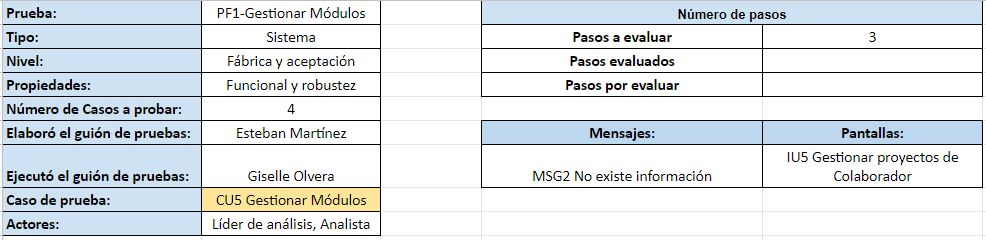
\includegraphics[width=.95\textwidth]{images/pruebas/diseno/encabezado}
		\caption{Ejemplo del encabezado de la matriz de pruebas}
		\label{fig:encabezado}
	\end{center}
\end{figure}

\begin{figure}[H]
	\begin{center}
		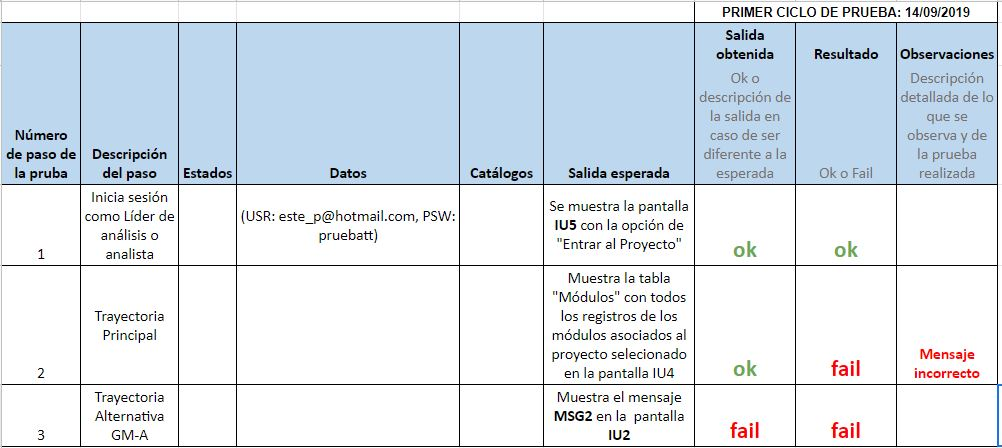
\includegraphics[width=.95\textwidth]{images/pruebas/diseno/tabla}
		\caption{Ejemplo de la estructura de la matriz de pruebas}
		\label{fig:estructura}
	\end{center}
\end{figure}

\subsubsection{REPORTE DE PRUEBAS SPRINT 1, 2 y 3 - CICLO 1}

Las pruebas contempladas para el primer ciclo de pruebas abarcan los Casos de Uso del Sprint 1, 2 y 3, Los cuales comprenden las siguientes gestiones:

\begin{itemize}
	\item CU1 Iniciar sesión.
	\item CU2 Gestionar proyectos de Administrador.
	\item CU3 Gestionar Colaboradores.
	\item CU4 Gestionar Proyectos de Colaborador.
\end{itemize}

Se realizaron pruebas dinámicas de sistema, con técnicas de caja negra.\\

Base de prueba:
\begin{itemize}
	\item Casos de Uso
	\item Especificaciónes de requisitos del sistema y software.
	\item Sistema y manual de usuario.
\end{itemize}

Objeto de prueba:
\begin{itemize}
	\item Sistema de software
\end{itemize}

\newpage

Los resultados finales del primer ciclo de prueba arrojaron los siguientes datos:

\begin{figure}[H]
	\begin{center}
		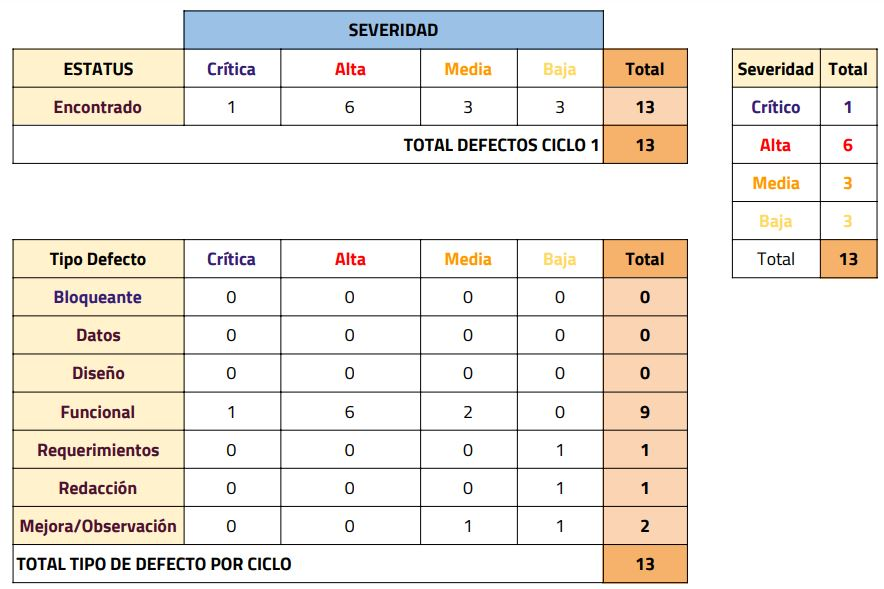
\includegraphics[width=.95\textwidth]{images/pruebas/s1c1}
		\caption{Informe de defectos Sprint 1, 2 y 3 Ciclo 1}
		\label{fig:infos1c1}
	\end{center}
\end{figure}

\newpage

\begin{figure}[H]
	\begin{center}
		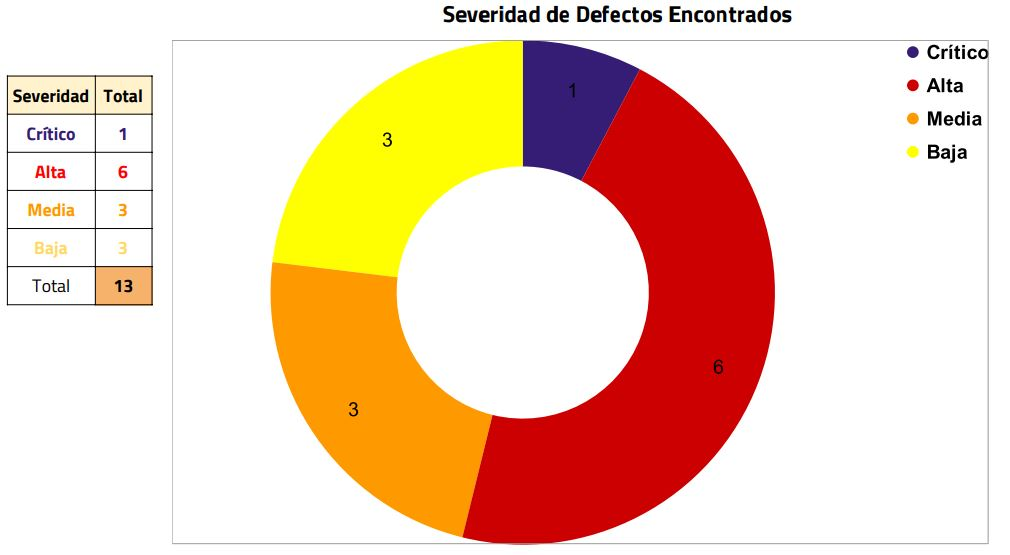
\includegraphics[width=.85\textwidth]{images/pruebas/s1c1-1}
		\caption{Gráfica de defectos por severidad Sprint 1, 2 y 3 Ciclo 1}
		\label{fig:infos1c1-1}
	\end{center}
\end{figure}

\begin{figure}[H]
	\begin{center}
		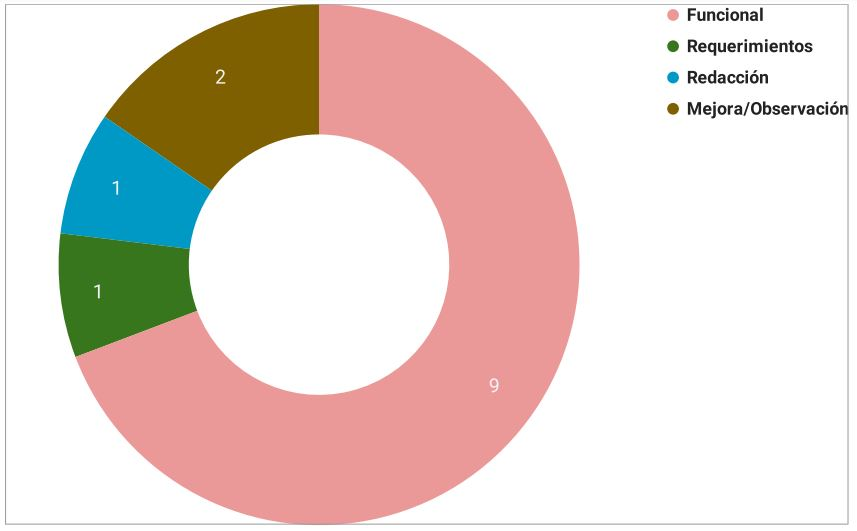
\includegraphics[width=.75\textwidth]{images/pruebas/s1c1-2}
		\caption{Gráfica de defectos por tipo de defecto Sprint 1, 2 y 3 Ciclo 1}
		\label{fig:infos1c1-2}
	\end{center}
\end{figure}

\newpage

\begin{figure}[H]
	\begin{center}
		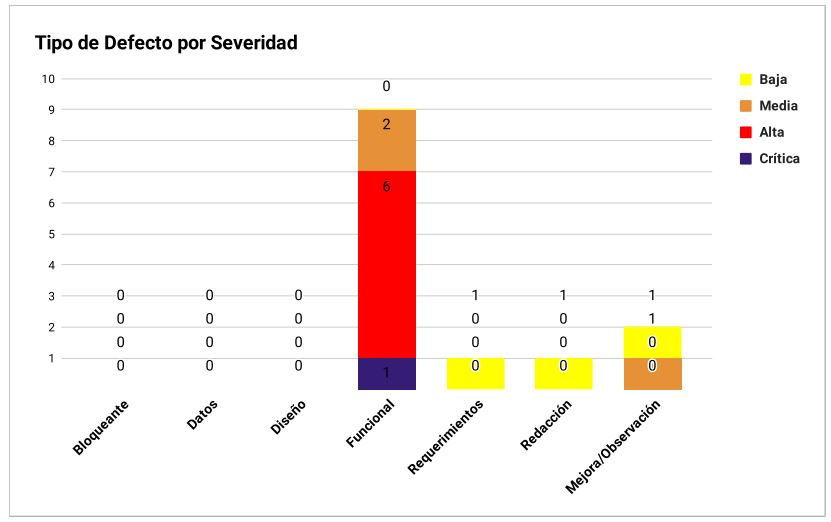
\includegraphics[width=.95\textwidth]{images/pruebas/s1c1-3}
		\caption{Gráfica de tipo de defectos por severidad Sprint 1, 2 y 3 Ciclo 1}
		\label{fig:infos1c1-3}
	\end{center}
\end{figure}

Se corrigieron los defectos encontrados en el primer ciclo.
\newpage

\subsubsection{REPORTE DE PRUEBAS SPRINT 4, 5 y 6 - CICLO 1}
Las pruebas contempladas para el segundo ciclo de pruebas abarcan los Casos de Uso del Sprint 4, 5 y 6, Los cuales comprenden las siguientes gestiones:

\begin{itemize}
	\item CU5 Gestionar Módulos.
	\item CU6 Gestionar Términos del glosario.
	\item CU7 Gestionar Entidades
\end{itemize}

Los resultados finales del primer ciclo de prueba arrojaron los siguientes datos:

\begin{figure}[H]
	\begin{center}
		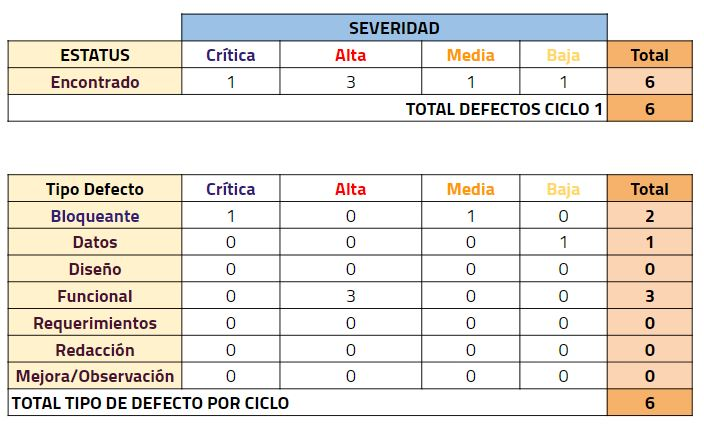
\includegraphics[width=.95\textwidth]{images/pruebas/s4c2}
		\caption{Informe de defectos Sprint 4, 5 y 6  Ciclo 1}
		\label{fig:infos4c2}
	\end{center}
\end{figure}

\begin{figure}[H]
	\begin{center}
		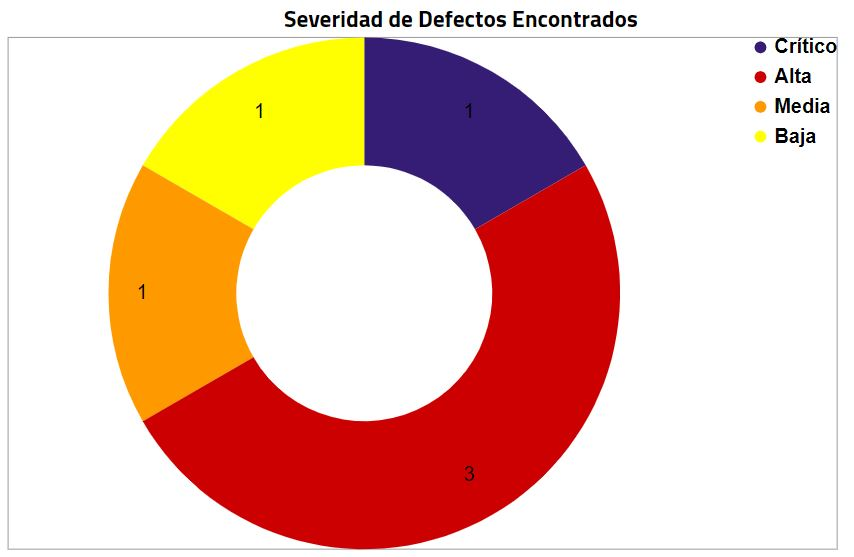
\includegraphics[width=.65\textwidth]{images/pruebas/s4c2-1}
		\caption{Gráfica de defectos por severidad Sprint 4, 5 y 6  Ciclo 1}
		\label{fig:infos4c2-1}
	\end{center}
\end{figure}

\begin{figure}[H]
	\begin{center}
		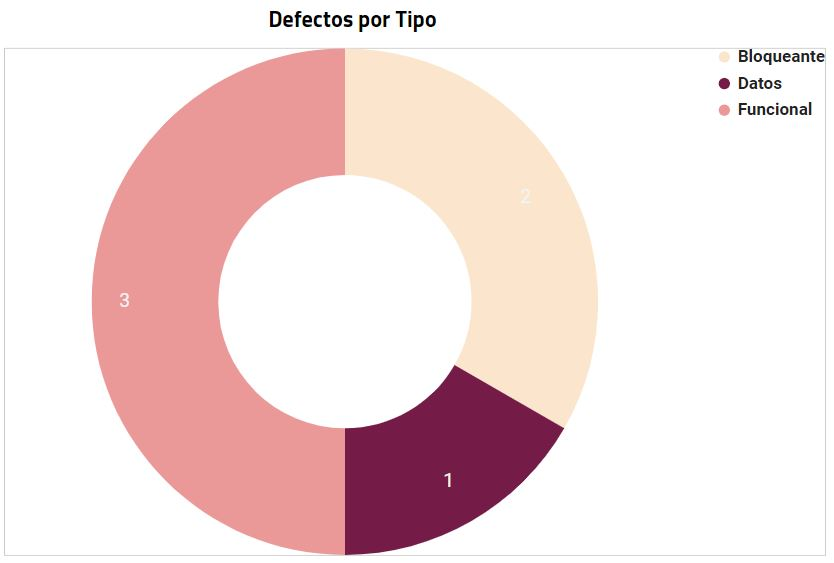
\includegraphics[width=.65\textwidth]{images/pruebas/s4c2-2}
		\caption{Gráfica de defectos por tipo de defecto Sprint 4, 5 y 6  Ciclo 1}
		\label{fig:infos4c2-2}
	\end{center}
\end{figure}

\subsubsection{REPORTE DE PRUEBAS SPRINT 7, 8 y 9 - CICLO 2}

Las pruebas contempladas para el segundo ciclo de pruebas abarcan los Casos de Uso del Sprint 7, 8 y 9, Los cuales comprenden las siguientes gestiones:

\begin{itemize}
	\item CU5 Gestionar Atributos.
	\item CU6 Gestionar Reglas de negocio.
	\item CU7 Gestionar Mensajes.
\end{itemize}

Los resultados finales del segundo ciclo de prueba arrojaron los siguientes datos:

\begin{figure}[H]
	\begin{center}
		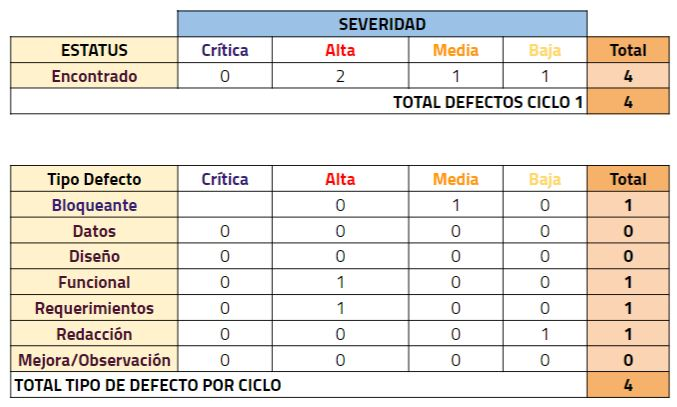
\includegraphics[width=.95\textwidth]{images/pruebas/s7c2}
		\caption{Informe de defectos Sprint 7, 8 y 9  Ciclo 2}
		\label{fig:infos7c2}
	\end{center}
\end{figure}

\begin{figure}[H]
	\begin{center}
		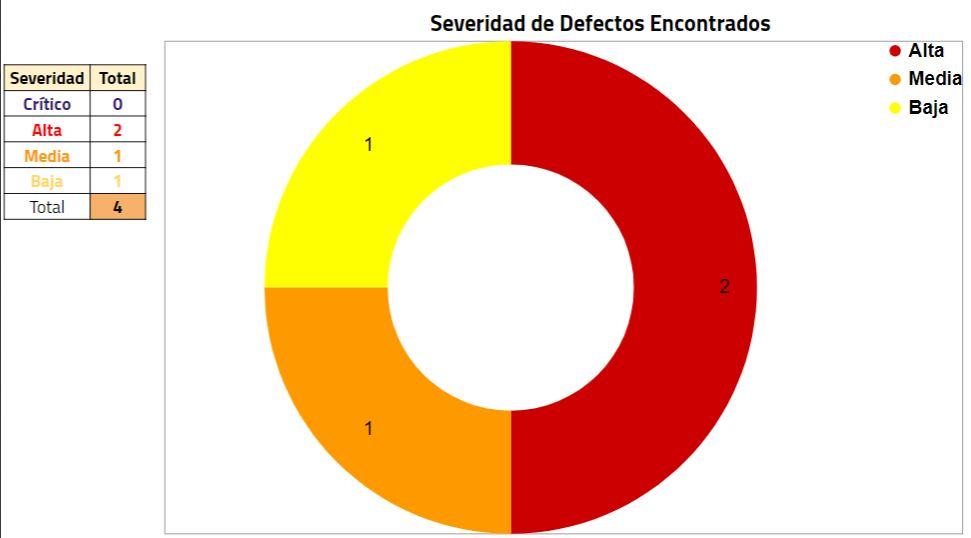
\includegraphics[width=.85\textwidth]{images/pruebas/s7c2-1}
		\caption{Gráfica de defectos por severidad Sprint 7, 8 y 9  Ciclo 2}
		\label{fig:infos7c2-1}
	\end{center}
\end{figure}

\begin{figure}[H]
	\begin{center}
		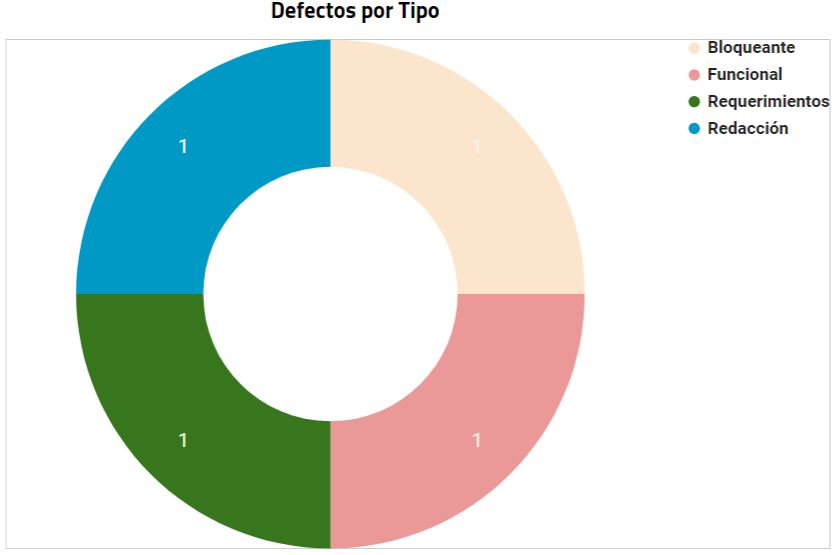
\includegraphics[width=.75\textwidth]{images/pruebas/s7c2-2}
		\caption{Gráfica de defectos por tipo de defecto Sprint 7, 8 y 9  Ciclo 2}
		\label{fig:infos7c2-2}
	\end{center}
\end{figure}

\subsubsection{REPORTE DE PRUEBAS SPRINT 10, 11 y 12 - CICLO 2}

Las pruebas contempladas para el segundo ciclo de pruebas abarcan los Casos de Uso del Sprint 10, 11 y 12, Los cuales comprenden las siguientes gestiones:

\begin{itemize}
	\item CU8 Gestionar Actores.
	\item CU9 Gestionar Pantallas.
	\item CU10 Gestionar Acciones.
\end{itemize}

Los resultados finales del segundo ciclo de prueba arrojaron los siguientes datos:

\begin{figure}[H]
	\begin{center}
		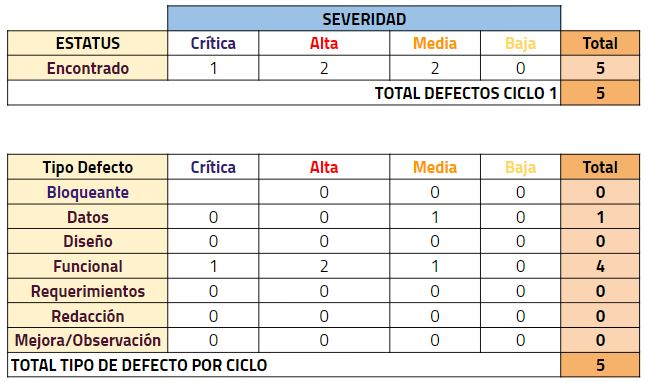
\includegraphics[width=.95\textwidth]{images/pruebas/s10c2}
		\caption{Informe de defectos Sprint 10, 11 y 12  Ciclo 2}
		\label{fig:infos10c2}
	\end{center}
\end{figure}

\begin{figure}[H]
	\begin{center}
		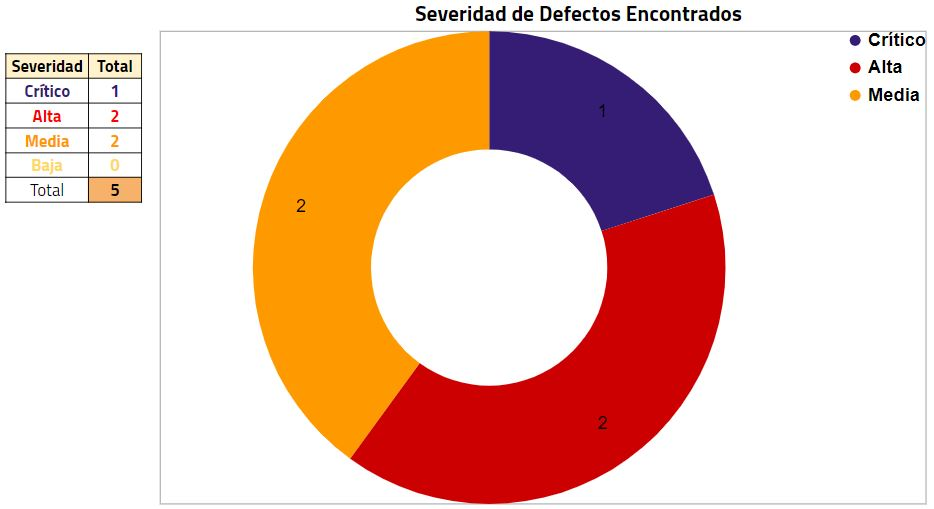
\includegraphics[width=.85\textwidth]{images/pruebas/s10c2-1}
		\caption{Gráfica de defectos por severidad Sprint 10, 11 y 12  Ciclo 2}
		\label{fig:infos10c2-1}
	\end{center}
\end{figure}

\begin{figure}[H]
	\begin{center}
		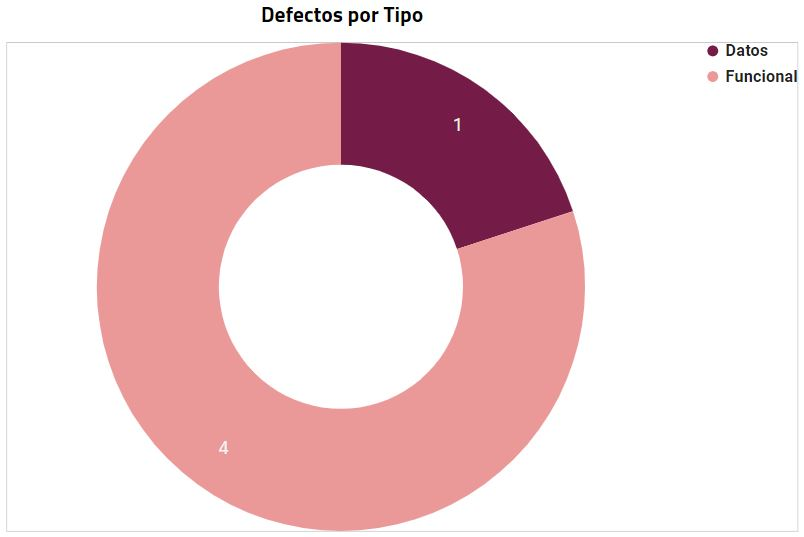
\includegraphics[width=.75\textwidth]{images/pruebas/s10c2-2}
		\caption{Gráfica de defectos por tipo de defecto 10, 11 y 12  Ciclo 2}
		\label{fig:infos10c2-2}
	\end{center}
\end{figure}

\subsubsection{REPORTE DE PRUEBAS SPRINT 13, 14 y 15 - CICLO 3}

Las pruebas contempladas para el tercer ciclo de pruebas abarcan los Casos de Uso del Sprint 13, 14 y 15, Los cuales comprenden las siguientes gestiones:

\begin{itemize}
	\item CU11.1.1 Gestionar Acciones.
	\item CU12.1.1 Gestionar Trayectorias.
	\item CU12.1.1.1 Gestionar Pasos.
\end{itemize}

Los resultados finales del segundo ciclo de prueba arrojaron los siguientes datos:

\begin{figure}[H]
	\begin{center}
		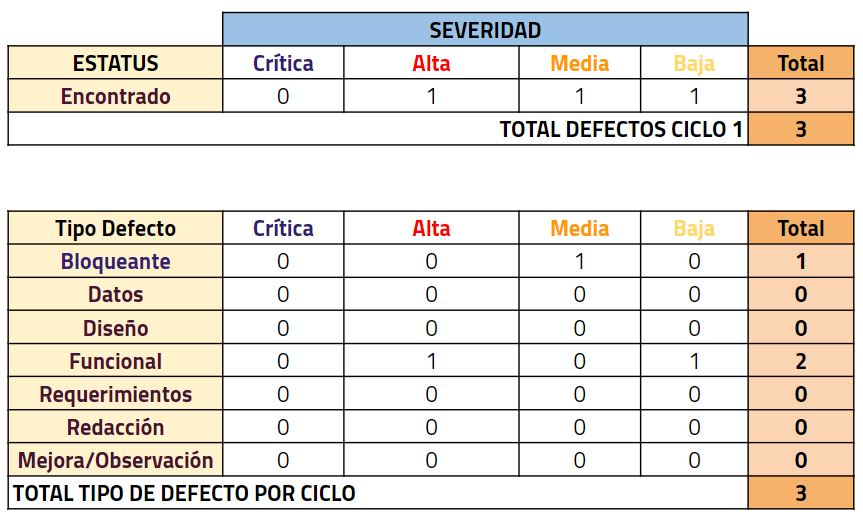
\includegraphics[width=.95\textwidth]{images/pruebas/s13c3}
		\caption{Informe de defectos Sprint 13, 14 y 15  Ciclo 3}
		\label{fig:infos13c3}
	\end{center}
\end{figure}

\begin{figure}[H]
	\begin{center}
		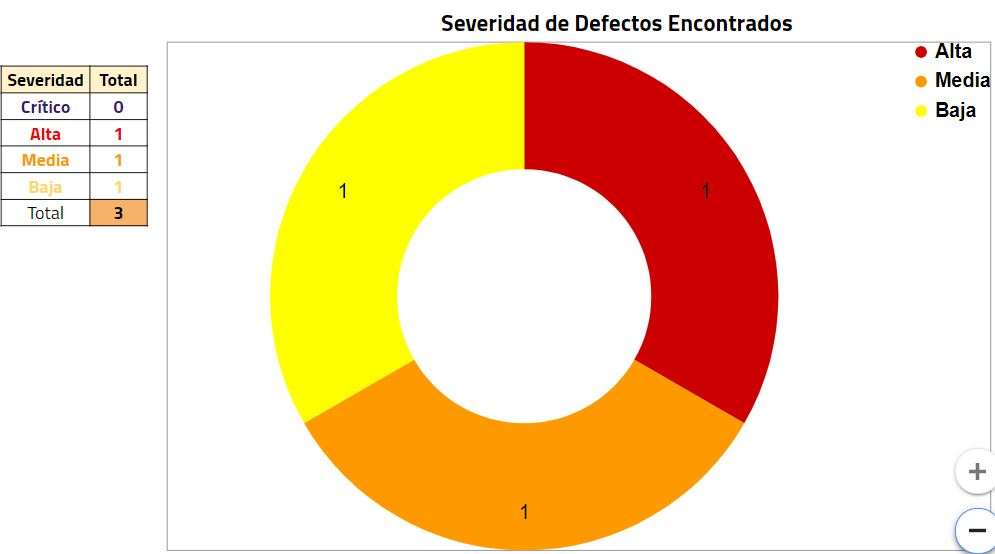
\includegraphics[width=.85\textwidth]{images/pruebas/s13c3-1}
		\caption{Gráfica de defectos por severidad Sprint 13, 14 y 15  Ciclo 3}
		\label{fig:infos13c3-1}
	\end{center}
\end{figure}

\begin{figure}[H]
	\begin{center}
		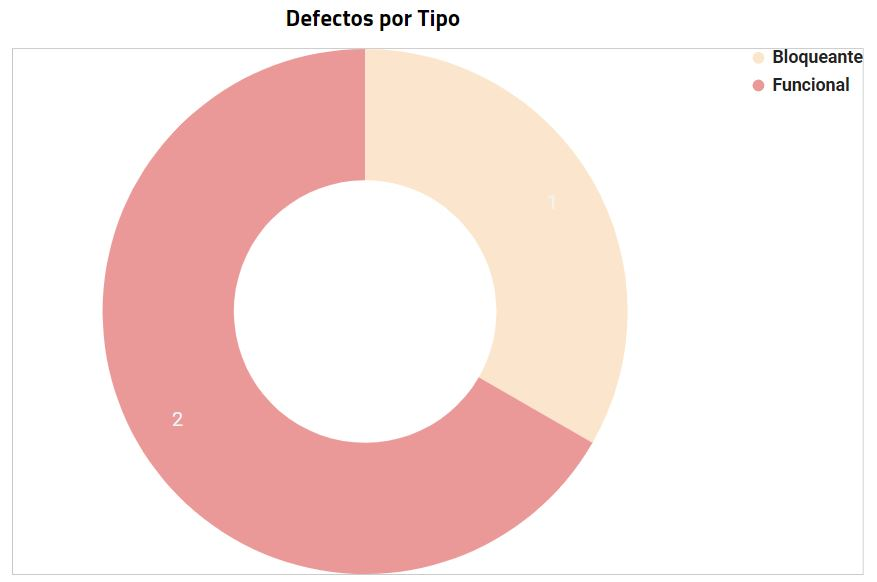
\includegraphics[width=.75\textwidth]{images/pruebas/s13c3-2}
		\caption{Gráfica de defectos por tipo de defecto 13, 14 y 15  Ciclo 3}
		\label{fig:infos13c3-2}
	\end{center}
\end{figure}

\section{Pruebas Estáticas}

Como se mencionó al inicio del capítulo, para obtener un producto de calidad no solo se deben realizar pruebas dinámicas, las pruebas estáticas también son necesarias. La herramienta sonarqube nos proporciona un análisis de código exhaustivo, los resultados que nos arrojó fueron los siguientes: \\

\begin{figure}[H]
	\begin{center}
		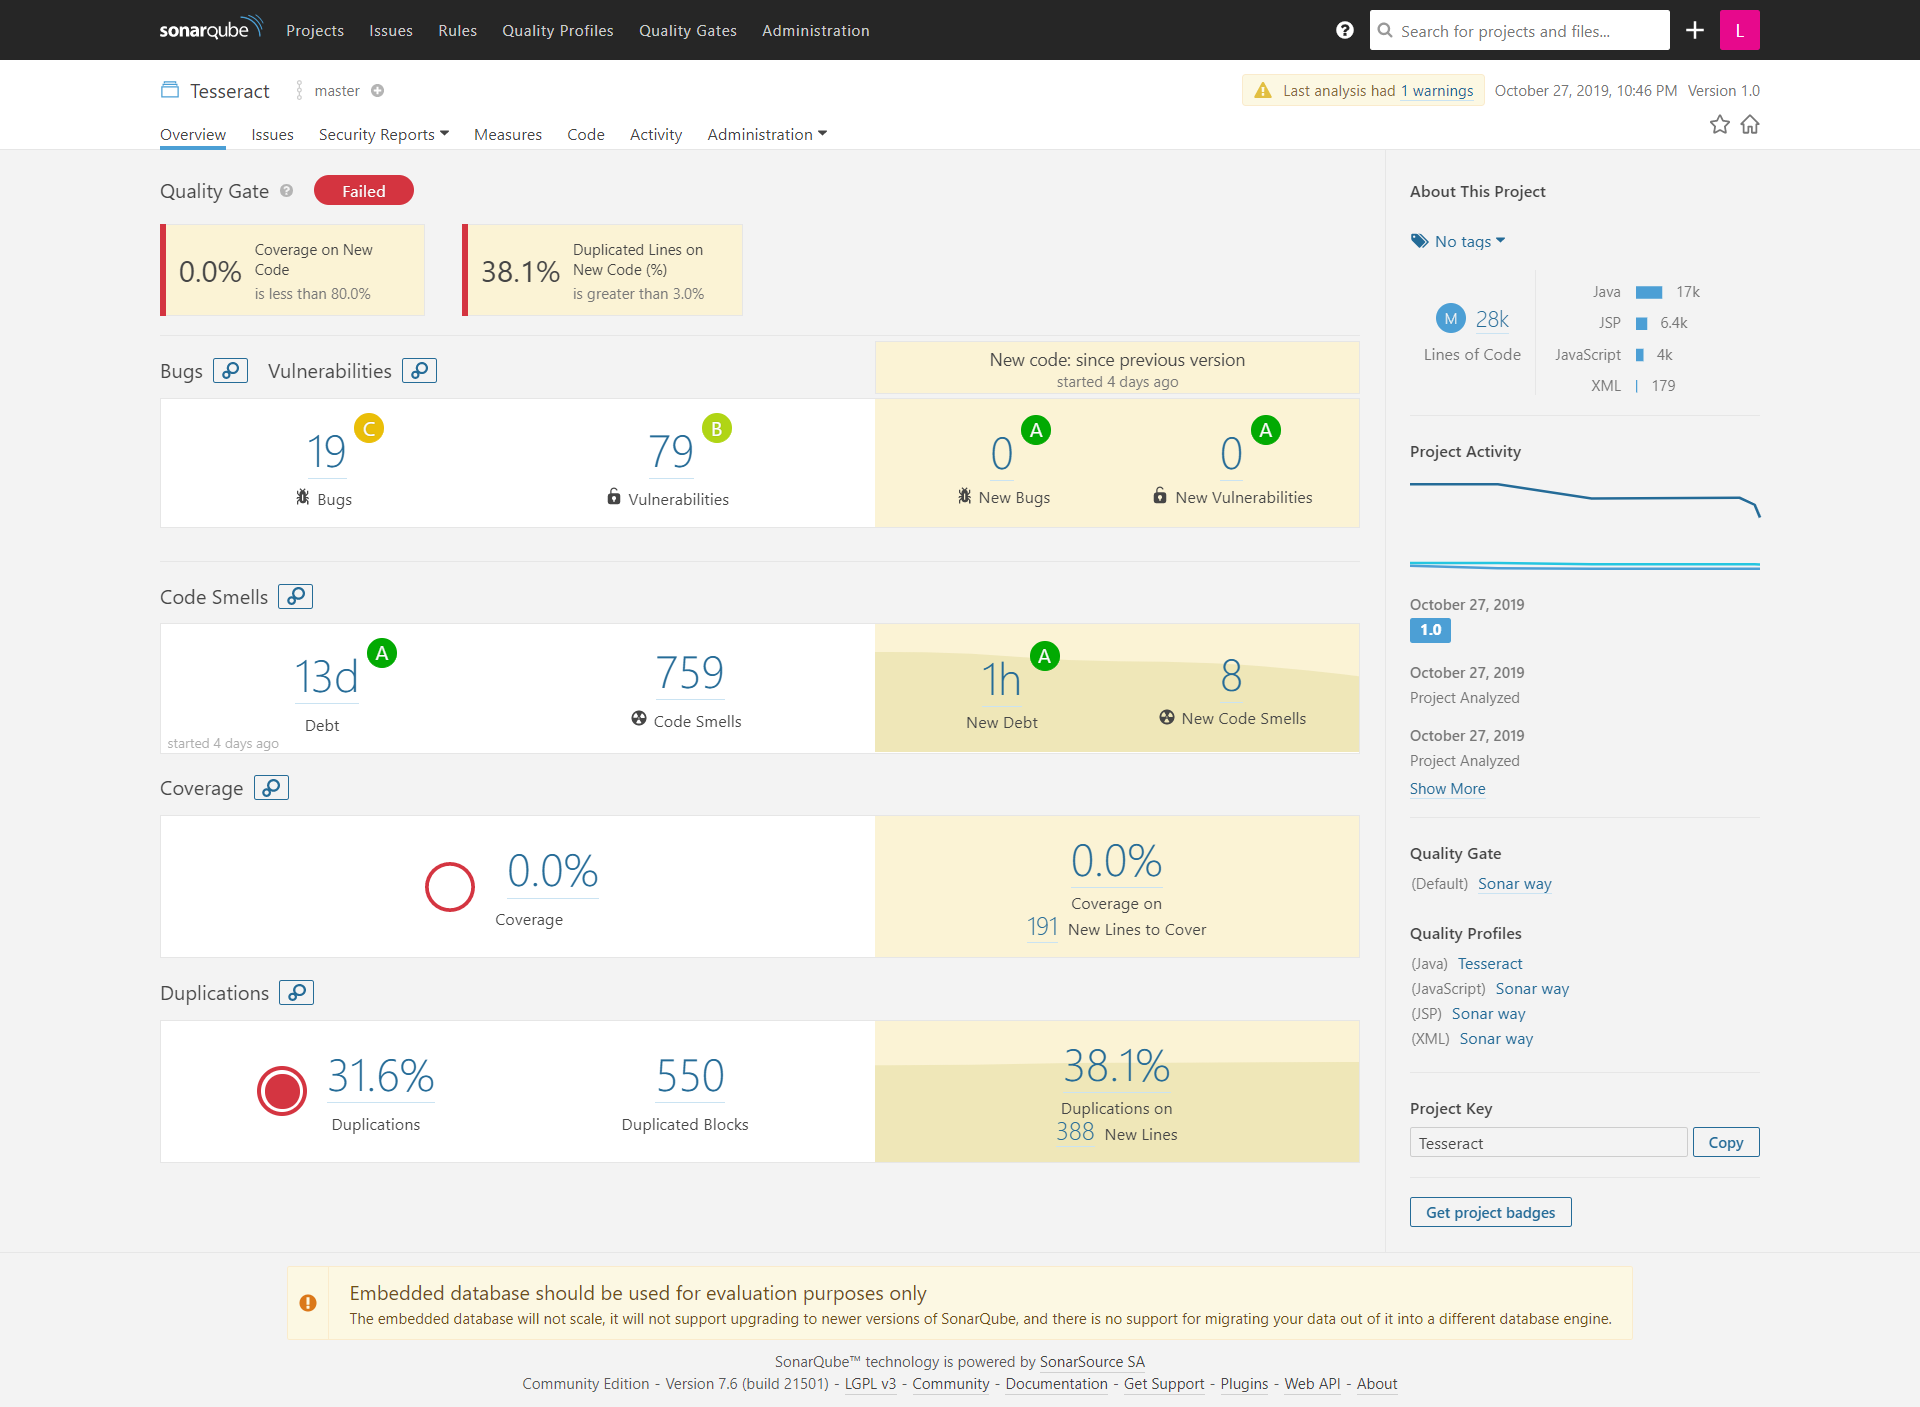
\includegraphics[width=.99\textwidth]{images/pruebas/estaticas/TesseractSonarFirstQualityTest}
		\caption{Reporte de pruebas estáticas SonarQube}
		\label{fig:infoesta}
	\end{center}
\end{figure}

%=========================================================
%=========================================================
\chapter{Bibliografía}

\begin{description}
	
		\item[\hypertarget{b01}{[1]}] Rui, K. Butler, G. (2003, April 21). Refactoring use case models: the metamodel [Online]. Available: https://dl.acm.org/citation.cfm?id=783140
		
		\item[\hypertarget{b02}{[2]}] Shuang, L. Sun, L. (2014, September 19). Automatic early defects detection in use case documents [Online]. Available: https://dl.acm.org/citation.cfm?id=2642969
		
		\item[\hypertarget{b03}{[3]}] 
		J. Lee. (1999, August). Analyzing user requirements use cases a goal driven approach. [Online]. Avaible: https://ieeexplore.ieee.org/document/776956
		
		\item[\hypertarget{b04}{[4]}]  L. Julijana. (2007, August). “Information Systems Modeling with Use Cases” IEEE Computer [Online]. Available:
		https://ieeexplore.ieee.org/document/4283759
		
		\item[\hypertarget{b05}{[5]}] Jason Gorman, J. G. (2007, 9 marzo). 10 Common Use Case Pitfalls. Recuperado 23 abril, 2018,  [Online]. Available: http://codemanship.co.uk/parlezuml/blog/?postid=364
		
		\item[\hypertarget{b06}{[6]}] Susan Lilly [2002, August]. “Use Case Pitfalls: Top 10 Problems from Real Projects Using Use Cases” [Online]. Avaible: https://ieeexplore.ieee.org/document/787547
		
		\item[\hypertarget{b07}{[7]}] Universidad Michoacana de San Nicolás de Hidalgo. (2014): “Competitividad y factores de éxito en empresas desarrolladoras de software” [Online]. Avaible: https://dialnet.unirioja.es/servlet/articulo?codigo=5101928
		
		\item[\hypertarget{b08}{[8]}] Mr. Vikas S. Chomal, Dr. Jatinderkumar R. Saini, (2014). “Significance of Software Documentation in Software
		Development Process“
 / (7 páginas). International Journal of Engineering Innovation and Research. 
		
		\item[\hypertarget{b09}{[9]}] Pressman, Roger. (2010). Ingenieria de Software. Un enfoque práctico / 7 ED.(777 páginas). USA: Mcgraw-Hill Interamericana.
		
		\item[\hypertarget{b10}{[10]}] B. Imran S. and H. Irfan, "UCD-generator - a LESSA application for use case design - IEEE Conference Publication", Ieeexplore.ieee.org, 2007. [Online]. \\Available: https://ieeexplore.ieee.org/document/4381333.
		
		\item[\hypertarget{b11}{[11]}] G. Booch, J. Rumbaugh, I. Jacobson, J. García Molina and J. Saez Martínez, El lenguaje unificado de modelado, 2nd ed. Madrid: Pearson Educación, 2010.
		
		\item[\hypertarget{b12}{[12]}] D. West, "Use Cases Considered Valuable (but Optional) For Lean/Agile Requirements Capture", InfoQ, 2010. [Online]. Available: https://www.infoq.com/news/2009/02/Use-Cases-Valuable-But-Optional. 
		
		\item[\hypertarget{b13}{[13]}] D. González, "Industria Mexicana del Software. Un estudio en cifras.", SG Buzz, 2005. [Online]. Available: https://sg.com.mx/revista/9/industria-mexicana-cifras. [Accessed: 20- Apr- 2019].
		
		\item[\hypertarget{b14}{[14]}] J. Gómez, "Métodos de Medición en Puntos Función (I): IFPUG FPA", El Laboratorio de las TI, 2014. [Online]. Available: https://www.laboratorioti.com/2013/01/16/metodos-de-medicion-en-puntos-funcion-i/. 
		
		\item[\hypertarget{b15}{[15]}] Ganesh Krishnamurthy, "CASE Tools 
		Adoption and Relevance" University of Missouri–St. Louis [Online]. Available: http://www.umsl.edu/~sauterv/analysis/F08papers/View.html
		
		\item[\hypertarget{b16}{[16]}] Annette L. du Plessis, A method for CASE tool evaluation, Information and Management, Volume 25, Issue 2, August 1993, Pages 93-102
		
		\item[\hypertarget{b17}{[17]}]	Erich Gamma, "Patrones de diseño: elementos de software orientado a objetos reutilizable", Pearson Educación, 2002. Addison-Wesley professional computing series.
		
		\item[\hypertarget{b18}{[18]}] IBM Knowledge Center, "Patrón de diseño de modelo-vista-controlador" [Online].\\ Available: https://www.ibm.com/support/knowledgecenter/es
		
		\item[\hypertarget{b19}{[19]}] Christopher Alexander, Sara Ishikawa, MurraySilverstein, Max Jacobson,
		Ingrid Fiksdahl-King, and Shlomo Angel.A Pattern Language. Oxford University
		Press, NewYork, 1977.
		
		\item[\hypertarget{b20}{[20]}] Glenn E. Krasner and Stephen T. Pope. A cookbook for using the model-view
		controller user interface paradigm in Smalltalk-80. Journal of Object-Oriented Programming, 1(3):26–49, August/September 1988.
		
		\item[\hypertarget{b21}{[21]}] BBVA-TRANSFORMACIÓN DIGITAL, "Metodología 'scrum': ¿Qué es un 'sprint'?", [Online].\\ Available: https://www.bbva.com/es/metodologia-scrum-que-es-un-sprint/
		
		\item[\hypertarget{b22}{[22]}] Proyectos Agiles, "Lista de tareas de la iteración (Sprint Backlog)", [Online].\\ Available: https://proyectosagiles.org/lista-tareas-iteracion-sprint-backlog/
		
		\item[\hypertarget{b23}{[23]}] Clemente Ruiz Durán, Michael Piore
		Andrew Schrkarn, "Los retos para el desarrollo
		de la industria del software", [Online].\\ Available: http://revistas.bancomext.gob.mx/rce/magazines/87/1/Ruiz-Schrank.pdf

		\item[\hypertarget{b24}{[24]}] Universidad Católica de los Angeles Chimbote-PERÚ, "Metodología de Desarrollo de Software"  [Online].\\ Available: https://www.uladech.edu.pe/images/stories/universidad/documentos/2018/metodologia-desarrollo-software-v001.pdf
		
		\item[\hypertarget{b25}{[25]}] (https://docs.spring.io/spring-framework/docs/current/spring-framework-reference/data-access.htmltransaction)
		
		\item[\hypertarget{b26}{[26]}] (https://docs.spring.io/spring-framework/docs/current/spring-framework-reference/data-access.htmltransaction-declarative)
		
		\item[\hypertarget{b27}{[27]}](https://struts.apache.org/birdseye.html) 
		
		\item[\hypertarget{b28}{[28]}] (https://docs.spring.io/spring/docs/3.0.0.M3/reference/html/ch04s04.htmlbeans-factory-scopes-singleton)

\end{description}
%=========================================================
%\chapter{Pruebas Ejecutadas} \label{cap:ocho}
Uno de los objetivos presentes en la entrega del trabajo terminal es obtener un producto de calidad y gran valor para el usuario final; para lograr este objetivo es necesario comprobar que cada segmento de la plataforma funcione de la manera esperada y que aporte valor al proceso de creación del documento. Por tal motivo se llevó a cabo la validación y verificación de cada sprint del sistema en la ejecucución de pruebas dinámicas correspondientes, de igual manera y con ayuda de la herramienta SonarQube el producto se sometió a pruebas de código en la ejecución de pruebas estáticas.

\section{Pruebas Dinámicas}

Con base en los enunciados de la ISTQB, se determinó que el nivel de prueba que se requiere para el trabajo terminal se concentra en las pruebas de sistema ya que el tiempo para ejecutar las pruebas es limitado en comparación con el tiempo de desarrollo y análisis; la ventaja de realizar las pruebas en este nivel es que se probará el funcionamiento del sistema completo así como la comunicación dentro de sus módulos.\\

El diseño de pruebas dinámicas está basado en la espeficicación técnica del sistema, la razón principal por la cual se aplicó esta técnica tiene que ver con el sustento documental con el que se cuenta.\\

\subsection{Diseño de Pruebas Dinámicas}

A continuación se detalla el diseño de las pruebas dinámicas basadas en la especificación técnica, así como de las herramientas creadas con base en el análisis de:

\begin{itemize}
	\item \textbf {Clases de equivalencia}
	\item \textbf {Valores frontera}
	\item \textbf {Reglas de negocio}
	\item \textbf {Máquinas de estado}
	\item \textbf {Casos de uso}
\end{itemize}

\subsubsection{Clases de equivalencia:}


\subsubsection{MATRICES DE PRUEBA}

Las matrices de pruebas son una herramienta que detalla el resultado de la ejecución de pruebas en comparación con cada una de las características y funcionalidades de los módulos del sistema. Están basadas en el documento de análisis, especifícamente en el documento de casos de uso.\\

Se implementaron las 5 técnicas 

La ejecución de pruebas se lleva a cabo una vez terminado el desarrollo de cada uno de los sprints estructurados en la metodología.\\

El objetivo de las matrices de prueba es validar y verificar a través de ciclos de pruebas que el producto cumpla con lo espeficicado en las etapas precedentes, en caso de que no se cumpla con las funcionalidades estipuladas o existan mejoras en su implementación se reporta una serie de defectos y sugerencias para que desarrollo se encargue de corregirlos; una vez que se solucionaron los problemas se ejecuta un ciclo de confirmación para comprobar que efectivamente se han corregido los defectos y que no se ha alterado ningúna otra parte del sistema.\\

A continuación se ilustra la estructura de las matrices de prueba que se diseñaron para registrar el resultado de su ejecución en los ciclos correspondientes.\\

\begin{figure}[H]
	\begin{center}
		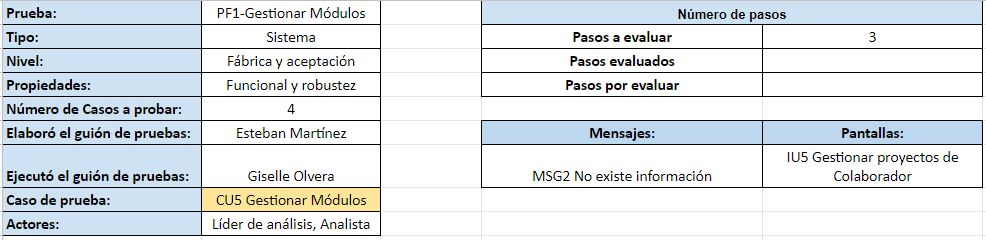
\includegraphics[width=.95\textwidth]{images/pruebas/diseno/encabezado}
		\caption{Ejemplo del encabezado de la matriz de pruebas}
		\label{fig:encabezado}
	\end{center}
\end{figure}

\begin{figure}[H]
	\begin{center}
		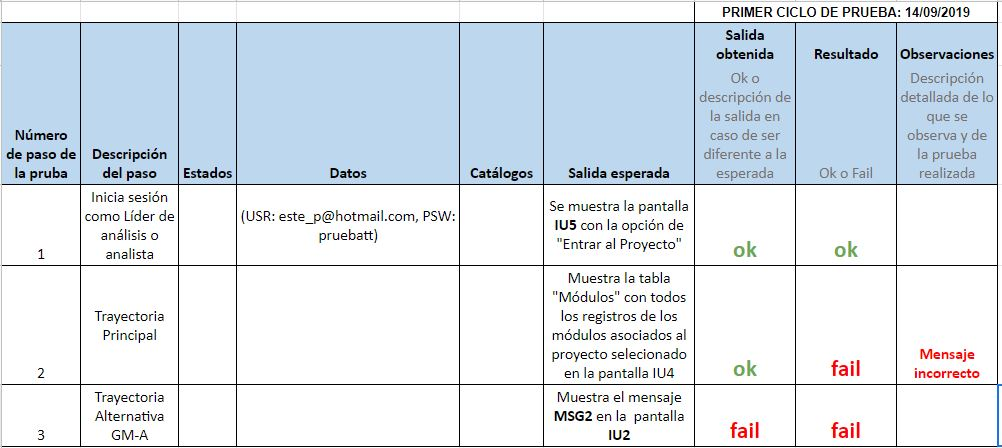
\includegraphics[width=.95\textwidth]{images/pruebas/diseno/tabla}
		\caption{Ejemplo de la estructura de la matriz de pruebas}
		\label{fig:estructura}
	\end{center}
\end{figure}

\subsubsection{REPORTE DE PRUEBAS SPRINT 1, 2 y 3 - CICLO 1}

Las pruebas contempladas para el primer ciclo de pruebas abarcan los Casos de Uso del Sprint 1, 2 y 3, Los cuales comprenden las siguientes gestiones:

\begin{itemize}
	\item CU1 Iniciar sesión.
	\item CU2 Gestionar proyectos de Administrador.
	\item CU3 Gestionar Colaboradores.
	\item CU4 Gestionar Proyectos de Colaborador.
\end{itemize}

Se realizaron pruebas dinámicas de sistema, con técnicas de caja negra.\\

Base de prueba:
\begin{itemize}
	\item Casos de Uso
	\item Especificaciónes de requisitos del sistema y software.
	\item Sistema y manual de usuario.
\end{itemize}

Objeto de prueba:
\begin{itemize}
	\item Sistema de software
\end{itemize}

\newpage

Los resultados finales del primer ciclo de prueba arrojaron los siguientes datos:

\begin{figure}[H]
	\begin{center}
		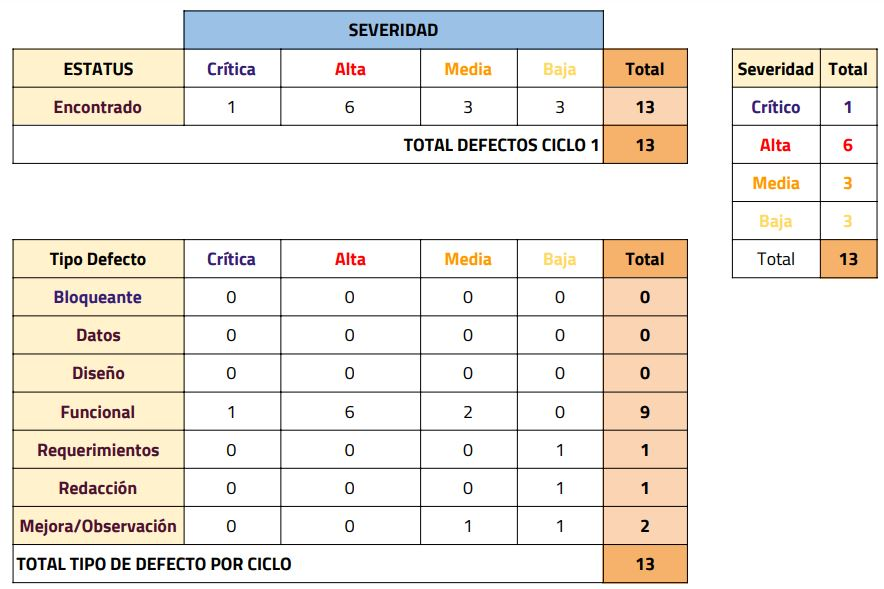
\includegraphics[width=.95\textwidth]{images/pruebas/s1c1}
		\caption{Informe de defectos Sprint 1, 2 y 3 Ciclo 1}
		\label{fig:infos1c1}
	\end{center}
\end{figure}

\newpage

\begin{figure}[H]
	\begin{center}
		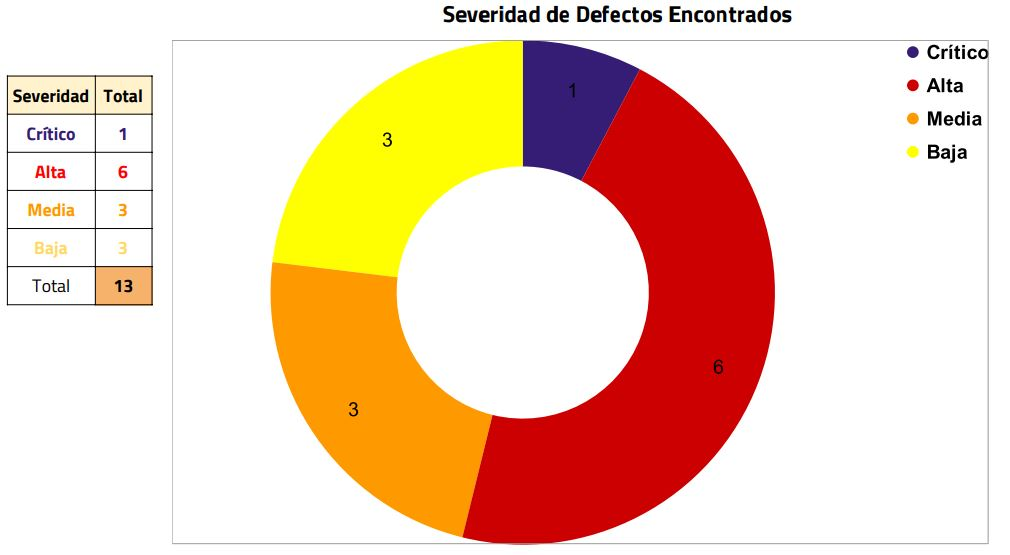
\includegraphics[width=.85\textwidth]{images/pruebas/s1c1-1}
		\caption{Gráfica de defectos por severidad Sprint 1, 2 y 3 Ciclo 1}
		\label{fig:infos1c1-1}
	\end{center}
\end{figure}

\begin{figure}[H]
	\begin{center}
		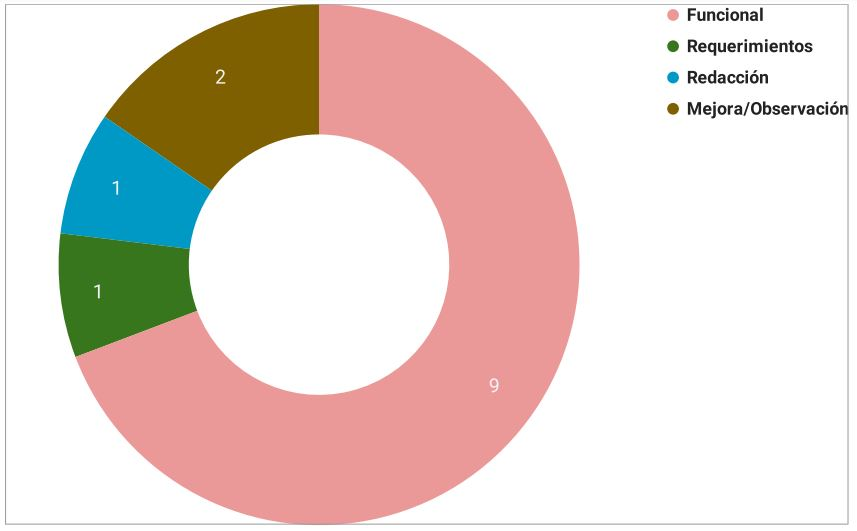
\includegraphics[width=.75\textwidth]{images/pruebas/s1c1-2}
		\caption{Gráfica de defectos por tipo de defecto Sprint 1, 2 y 3 Ciclo 1}
		\label{fig:infos1c1-2}
	\end{center}
\end{figure}

\newpage

\begin{figure}[H]
	\begin{center}
		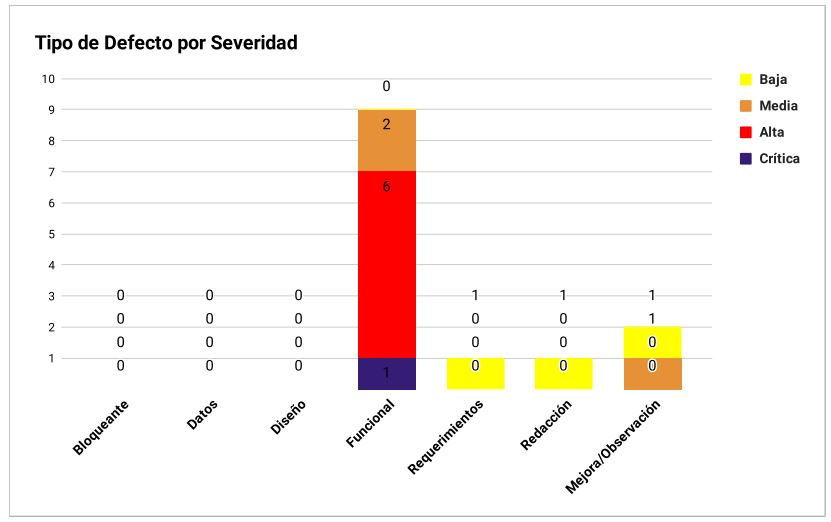
\includegraphics[width=.95\textwidth]{images/pruebas/s1c1-3}
		\caption{Gráfica de tipo de defectos por severidad Sprint 1, 2 y 3 Ciclo 1}
		\label{fig:infos1c1-3}
	\end{center}
\end{figure}

Se corrigieron los defectos encontrados en el primer ciclo.
\newpage

\subsubsection{REPORTE DE PRUEBAS SPRINT 4, 5 y 6 - CICLO 1}
Las pruebas contempladas para el segundo ciclo de pruebas abarcan los Casos de Uso del Sprint 4, 5 y 6, Los cuales comprenden las siguientes gestiones:

\begin{itemize}
	\item CU5 Gestionar Módulos.
	\item CU6 Gestionar Términos del glosario.
	\item CU7 Gestionar Entidades
\end{itemize}

Los resultados finales del primer ciclo de prueba arrojaron los siguientes datos:

\begin{figure}[H]
	\begin{center}
		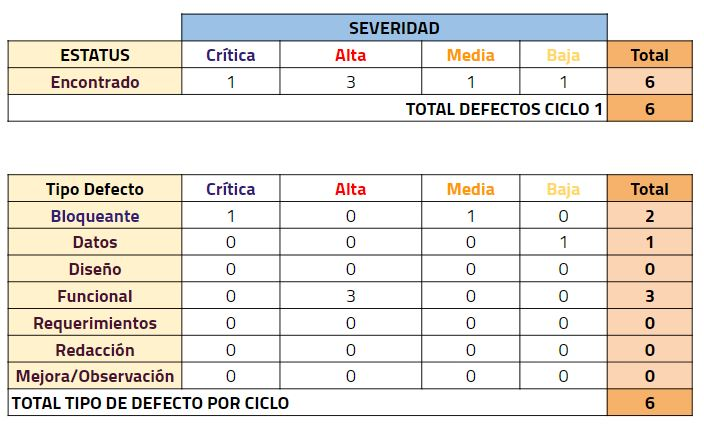
\includegraphics[width=.95\textwidth]{images/pruebas/s4c2}
		\caption{Informe de defectos Sprint 4, 5 y 6  Ciclo 1}
		\label{fig:infos4c2}
	\end{center}
\end{figure}

\begin{figure}[H]
	\begin{center}
		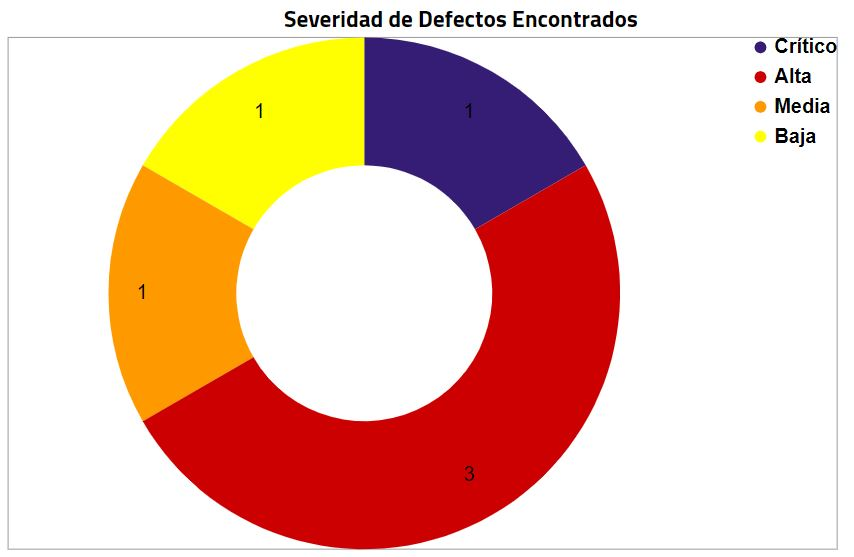
\includegraphics[width=.65\textwidth]{images/pruebas/s4c2-1}
		\caption{Gráfica de defectos por severidad Sprint 4, 5 y 6  Ciclo 1}
		\label{fig:infos4c2-1}
	\end{center}
\end{figure}

\begin{figure}[H]
	\begin{center}
		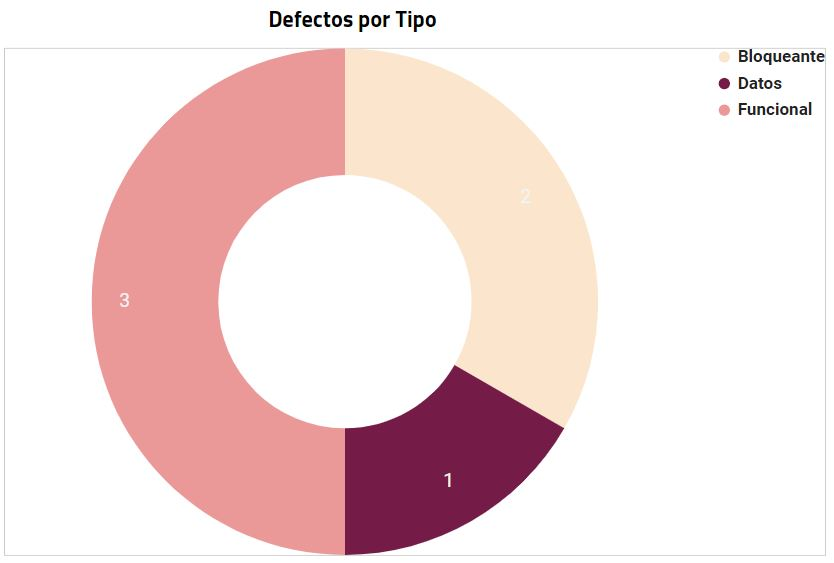
\includegraphics[width=.65\textwidth]{images/pruebas/s4c2-2}
		\caption{Gráfica de defectos por tipo de defecto Sprint 4, 5 y 6  Ciclo 1}
		\label{fig:infos4c2-2}
	\end{center}
\end{figure}

\subsubsection{REPORTE DE PRUEBAS SPRINT 7, 8 y 9 - CICLO 2}

Las pruebas contempladas para el segundo ciclo de pruebas abarcan los Casos de Uso del Sprint 7, 8 y 9, Los cuales comprenden las siguientes gestiones:

\begin{itemize}
	\item CU5 Gestionar Atributos.
	\item CU6 Gestionar Reglas de negocio.
	\item CU7 Gestionar Mensajes.
\end{itemize}

Los resultados finales del segundo ciclo de prueba arrojaron los siguientes datos:

\begin{figure}[H]
	\begin{center}
		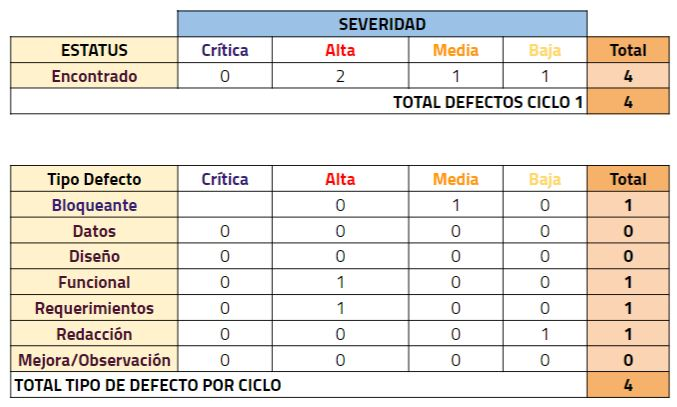
\includegraphics[width=.95\textwidth]{images/pruebas/s7c2}
		\caption{Informe de defectos Sprint 7, 8 y 9  Ciclo 2}
		\label{fig:infos7c2}
	\end{center}
\end{figure}

\begin{figure}[H]
	\begin{center}
		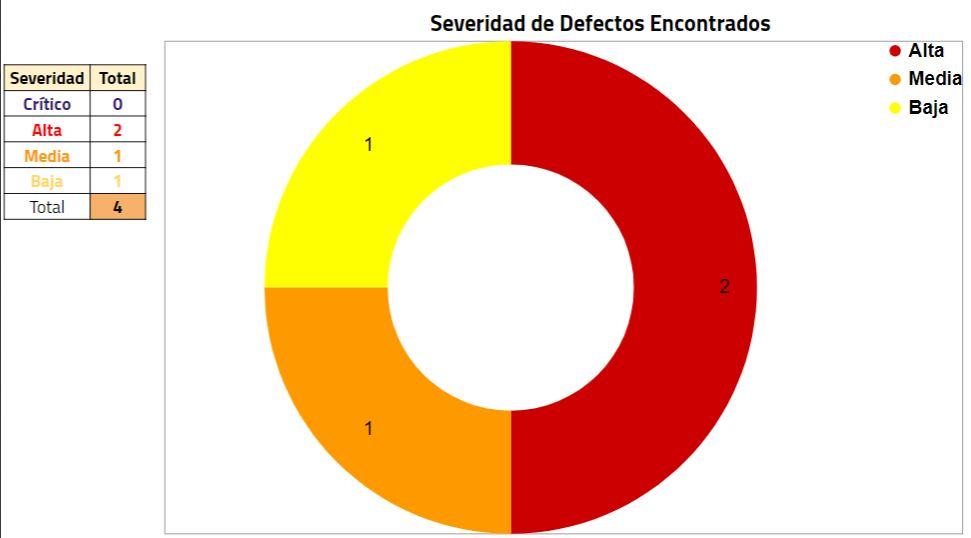
\includegraphics[width=.85\textwidth]{images/pruebas/s7c2-1}
		\caption{Gráfica de defectos por severidad Sprint 7, 8 y 9  Ciclo 2}
		\label{fig:infos7c2-1}
	\end{center}
\end{figure}

\begin{figure}[H]
	\begin{center}
		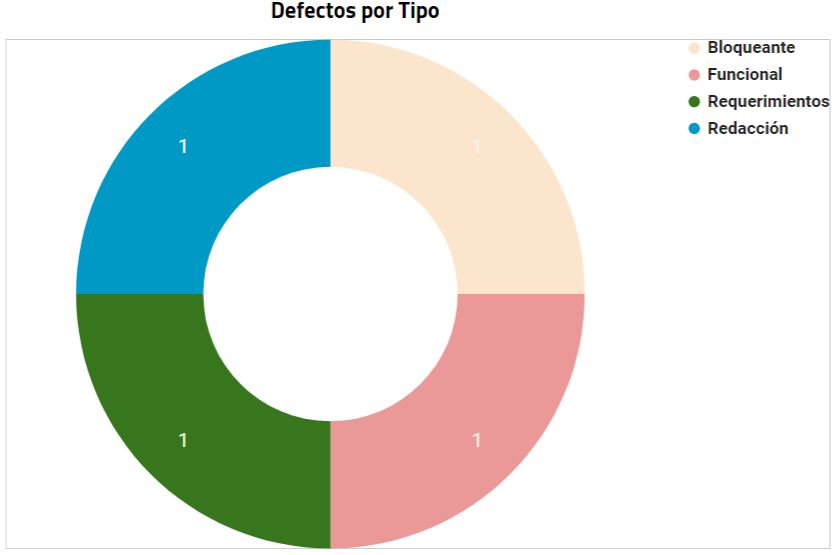
\includegraphics[width=.75\textwidth]{images/pruebas/s7c2-2}
		\caption{Gráfica de defectos por tipo de defecto Sprint 7, 8 y 9  Ciclo 2}
		\label{fig:infos7c2-2}
	\end{center}
\end{figure}

\subsubsection{REPORTE DE PRUEBAS SPRINT 10, 11 y 12 - CICLO 2}

Las pruebas contempladas para el segundo ciclo de pruebas abarcan los Casos de Uso del Sprint 10, 11 y 12, Los cuales comprenden las siguientes gestiones:

\begin{itemize}
	\item CU8 Gestionar Actores.
	\item CU9 Gestionar Pantallas.
	\item CU10 Gestionar Acciones.
\end{itemize}

Los resultados finales del segundo ciclo de prueba arrojaron los siguientes datos:

\begin{figure}[H]
	\begin{center}
		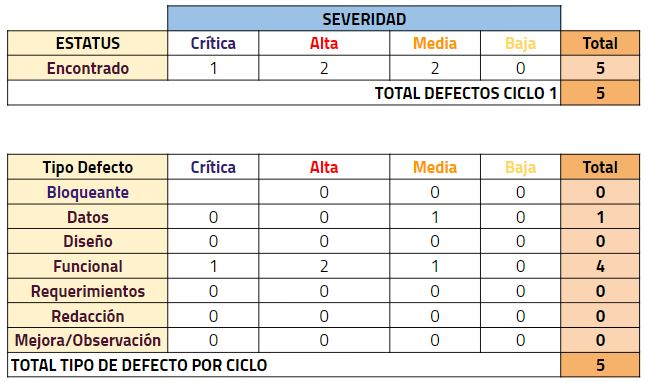
\includegraphics[width=.95\textwidth]{images/pruebas/s10c2}
		\caption{Informe de defectos Sprint 10, 11 y 12  Ciclo 2}
		\label{fig:infos10c2}
	\end{center}
\end{figure}

\begin{figure}[H]
	\begin{center}
		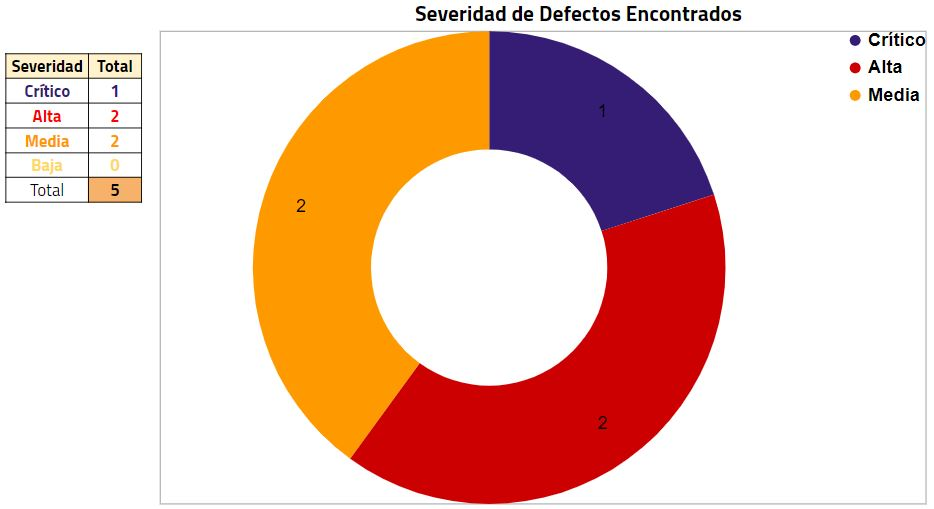
\includegraphics[width=.85\textwidth]{images/pruebas/s10c2-1}
		\caption{Gráfica de defectos por severidad Sprint 10, 11 y 12  Ciclo 2}
		\label{fig:infos10c2-1}
	\end{center}
\end{figure}

\begin{figure}[H]
	\begin{center}
		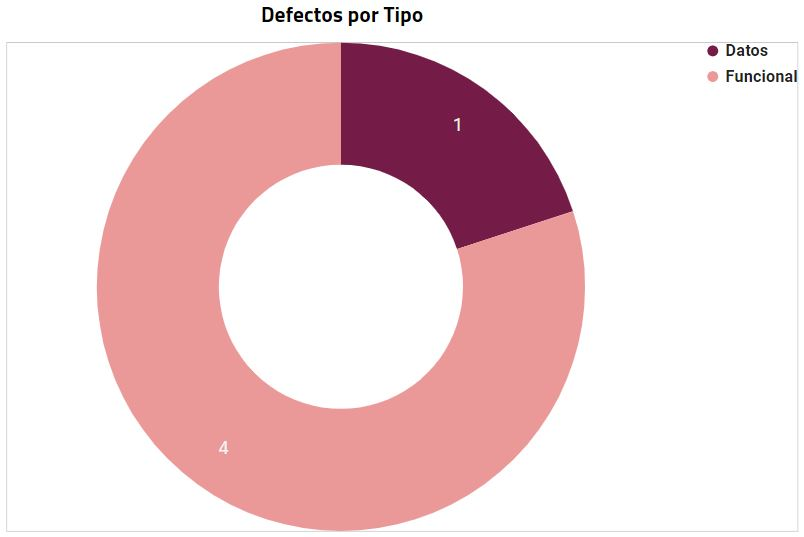
\includegraphics[width=.75\textwidth]{images/pruebas/s10c2-2}
		\caption{Gráfica de defectos por tipo de defecto 10, 11 y 12  Ciclo 2}
		\label{fig:infos10c2-2}
	\end{center}
\end{figure}

\subsubsection{REPORTE DE PRUEBAS SPRINT 13, 14 y 15 - CICLO 3}

Las pruebas contempladas para el tercer ciclo de pruebas abarcan los Casos de Uso del Sprint 13, 14 y 15, Los cuales comprenden las siguientes gestiones:

\begin{itemize}
	\item CU11.1.1 Gestionar Acciones.
	\item CU12.1.1 Gestionar Trayectorias.
	\item CU12.1.1.1 Gestionar Pasos.
\end{itemize}

Los resultados finales del segundo ciclo de prueba arrojaron los siguientes datos:

\begin{figure}[H]
	\begin{center}
		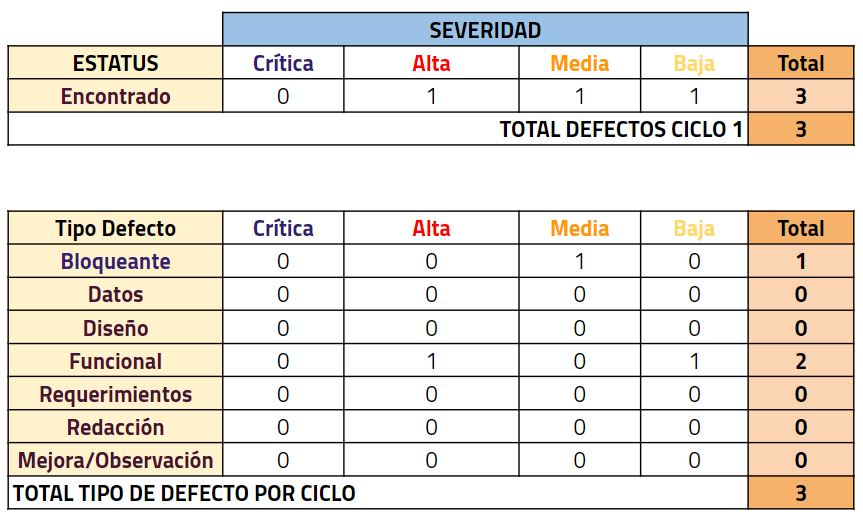
\includegraphics[width=.95\textwidth]{images/pruebas/s13c3}
		\caption{Informe de defectos Sprint 13, 14 y 15  Ciclo 3}
		\label{fig:infos13c3}
	\end{center}
\end{figure}

\begin{figure}[H]
	\begin{center}
		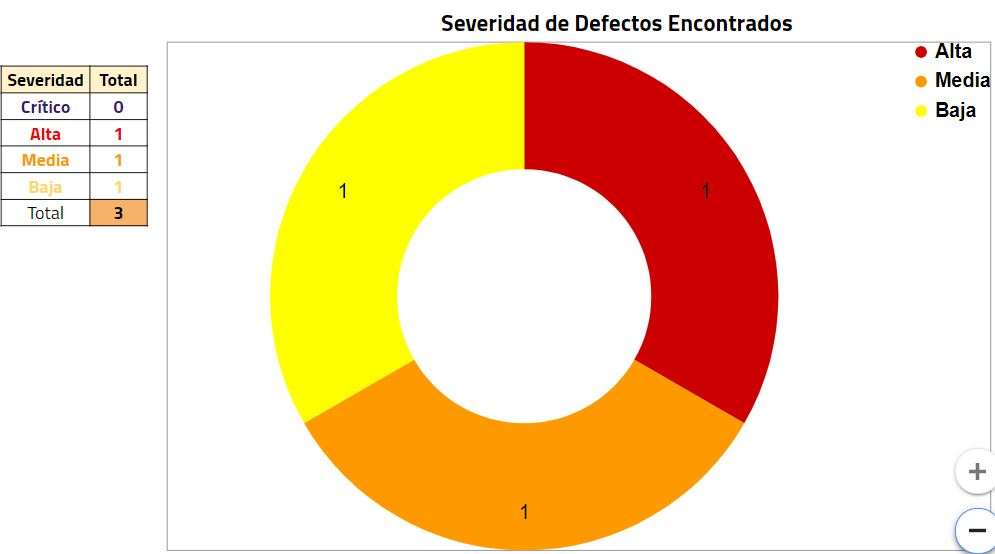
\includegraphics[width=.85\textwidth]{images/pruebas/s13c3-1}
		\caption{Gráfica de defectos por severidad Sprint 13, 14 y 15  Ciclo 3}
		\label{fig:infos13c3-1}
	\end{center}
\end{figure}

\begin{figure}[H]
	\begin{center}
		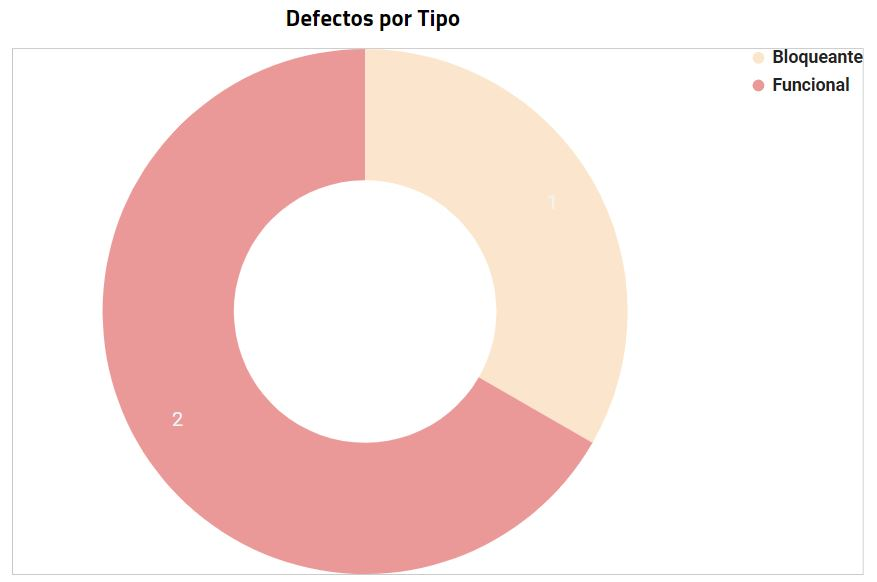
\includegraphics[width=.75\textwidth]{images/pruebas/s13c3-2}
		\caption{Gráfica de defectos por tipo de defecto 13, 14 y 15  Ciclo 3}
		\label{fig:infos13c3-2}
	\end{center}
\end{figure}

\section{Pruebas Estáticas}

Como se mencionó al inicio del capítulo, para obtener un producto de calidad no solo se deben realizar pruebas dinámicas, las pruebas estáticas también son necesarias. La herramienta sonarqube nos proporciona un análisis de código exhaustivo, los resultados que nos arrojó fueron los siguientes: \\

\begin{figure}[H]
	\begin{center}
		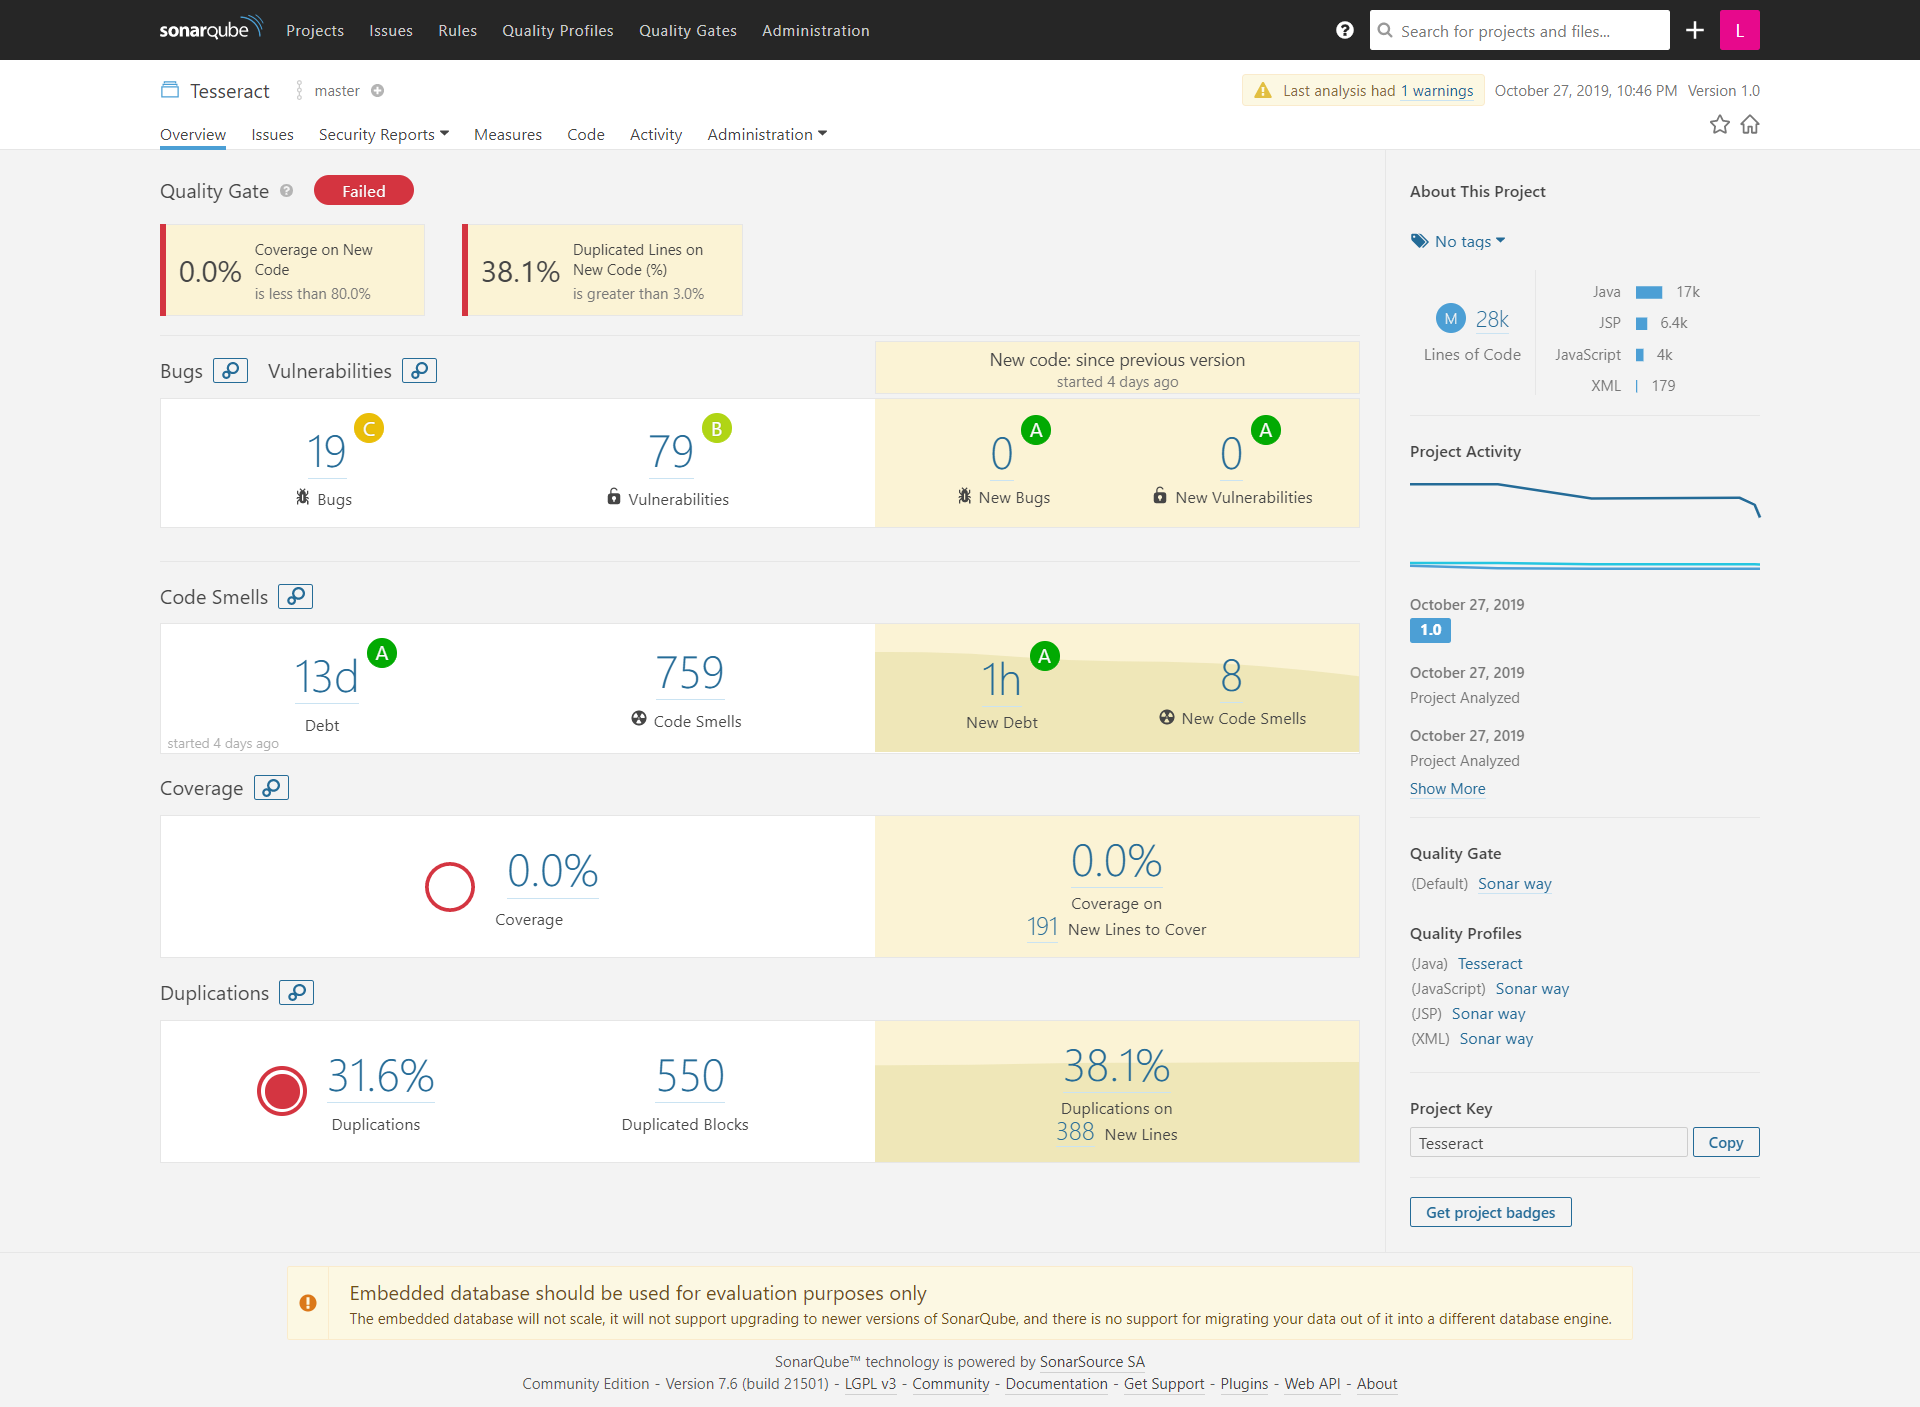
\includegraphics[width=.99\textwidth]{images/pruebas/estaticas/TesseractSonarFirstQualityTest}
		\caption{Reporte de pruebas estáticas SonarQube}
		\label{fig:infoesta}
	\end{center}
\end{figure}

\end{document}

